\documentclass[letterpaper,11pt]{article}

\usepackage[utf8]{inputenc}
\usepackage[spanish]{babel}
\usepackage[
    letterpaper,
    top=1.5cm,
    bottom=2cm,
    left=2cm,
    right=2cm
]{geometry}

\usepackage{graphicx}
\usepackage{fancyhdr}
\usepackage[table,xcdraw]{xcolor}
\usepackage{tikz}
\usetikzlibrary{shapes.geometric, arrows, positioning, fit, backgrounds, calc, babel}
\usepackage{ifpdf}
\usepackage{blindtext}
\usepackage[cmex10]{amsmath}
\usepackage{amssymb}
\usepackage{amsfonts}
\usepackage{float}
\usepackage{siunitx}
\usepackage{listings}
\usepackage{hyperref}
\usepackage{subcaption}
\usepackage{booktabs}
\usepackage{url}
\usepackage{wrapfig}
\usepackage{titlesec}
\usepackage[export]{adjustbox}
\usepackage{imakeidx}
\usepackage{parskip}
\usepackage[numbers]{natbib}

\usepackage{ragged2e}
\usepackage{setspace}
\usepackage{array}
\usepackage{longtable}

% Definición de un nuevo tipo de columna para evitar "Underfull \hbox" en tablas
\newcolumntype{L}[1]{>{\RaggedRight\arraybackslash}p{#1}}

\hypersetup{colorlinks=false,bookmarksopen=true,linkbordercolor={1 1 1}}

\newcommand{\rfigura}[1]{Fig.\ref{#1}}
\newcommand{\rtabla}[1]{Tabla \ref{#1}}

% Datos del informe
\newcommand{\Curso}{IEE2913 --- Diseño Eléctrico (Capstone)}
\newcommand{\TituloInforme}{Informe de Planificación: Arquitectura del Hardware/Software}
\newcommand{\NumeroGrupo}{10}
\newcommand{\NombreProyecto}{SupaClock: Wearable Biométrico Modular}
\newcommand{\Integrantes}{Tomás Avendaño, Benjamín Sepúlveda, Pablo Uribe}
\newcommand{\FechaEntrega}{25 de marzo de 2026}

\lstset{
  basicstyle=\ttfamily\small,
  breaklines=true,
  breakatwhitespace=true,
  postbreak=\mbox{\textcolor{red}{$\hookrightarrow$}\space},
  captionpos=b,
  frame=single,
  numbers=left,
  numberstyle=\tiny\color{gray}
}

\begin{document}

% Encabezado manual
\noindent
\begin{minipage}[c]{0.12\textwidth}
    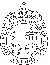
\includegraphics[width=0.9\linewidth]{logo.pdf}
    \vspace{1cm} % Placeholder para el logo
\end{minipage}
\hfill
\begin{minipage}[c]{0.68\textwidth}
    \small
    PONTIFICIA UNIVERSIDAD CATÓLICA DE CHILE\\
    ESCUELA DE INGENIERÍA\\
    Departamento de Ingeniería Eléctrica\\
    \Curso
\end{minipage}
\hfill
\begin{minipage}[c]{0.15\textwidth}
    \raggedleft
    \small
    Grupo \NumeroGrupo
\end{minipage}

\vspace{0.5cm}

\begin{center}
    {\Large \textbf{\TituloInforme}}\\[0.5cm]
\end{center}

\noindent
\textbf{Proyecto:} \NombreProyecto\\
\textbf{Integrantes:} \Integrantes\\
\textbf{Fecha:} \FechaEntrega

% Pie de página
\pagestyle{fancy}
\fancyhf{}
\renewcommand{\headrulewidth}{0pt}
\fancyfoot[RO,LE]{\thepage}
\lfoot{IEE2913}
\fancyfoot[C]{Diseño Eléctrico}
\renewcommand{\footrulewidth}{0.4pt}

\vspace{5mm}
\hrule
\vspace{5mm}
\tableofcontents
\newpage
\listoffigures
\vspace{1cm}
\listoftables
\newpage

% ==========================================
% 1. CONTEXTO Y OBJETIVOS
% ==========================================
\section{Contexto y Objetivos}

% Esta brecha se mantiene en la población adulta, donde el 49,7% de los hombres mayores de 18 años se declara activo, en comparación con solo un 40,3% de las mujeres
%https://www.ciperchile.cl/2025/05/24/resultados-de-la-encuesta-nacional-de-actividad-fisica-y-deporte-una-oportunidad-para-fortalecer-el-bienestar-integral-en-chile/


%https://www.ucchristus.cl/blog-salud-uc/articulos/2025/5-razones-por-las-que-chile-es-el-pa%C3%ADs-con-m%C3%A1s-obesidad-de-latinoam%C3%A9rica 

Según la Encuesta Nacional de Actividad Física \citep{encuesta_af}, apenas un 49.7\% de los hombres y un 40.3\% de las mujeres mayores de 18 años en el país mantienen un nivel de actividad física adecuado. Esta cifra resulta alarmante al considerar que el 42\% de la población adulta presenta sobrepeso \citep{obesidad_chile}, un factor de riesgo determinante para el desarrollo de patologías crónicas a largo plazo. Frente a este escenario, surge la necesidad de fomentar hábitos de vida más saludables. Con el fin de contribuir a esta problemática, el presente proyecto propone el diseño y desarrollo de un dispositivo \textit{wearable} de bajo costo que permita a los usuarios monitorizar sus variables biométricas y registrar su evolución física de manera accesible.

\section{Posibles soluciones ante la problemática}
Para cumplir con los requerimientos solicitados por el cliente, planteamos dos posibles soluciones. Cada una de ellas con ventajas y desventajas en distintos ámbitos.

\subsection{Peto deportivo inteligente}
Con el fin de proponer una solución que sea poco visible y sea más fácil de utilizar al momento de realizar deporte, planteamos la posibilidad de diseñar un peto deportivo que integrara los distintos sensores y tuviera una pantalla en el pecho. La \rfigura{fig:peto} ilustra un peto deportivo comercial que se utilizó como referencia de este concepto: una prenda ceñida al torso que podría alojar sensores distribuidos sobre el pecho, aprovechando la cercanía al corazón y la estabilidad del contacto con la piel.

\begin{figure}[h]
    \centering
    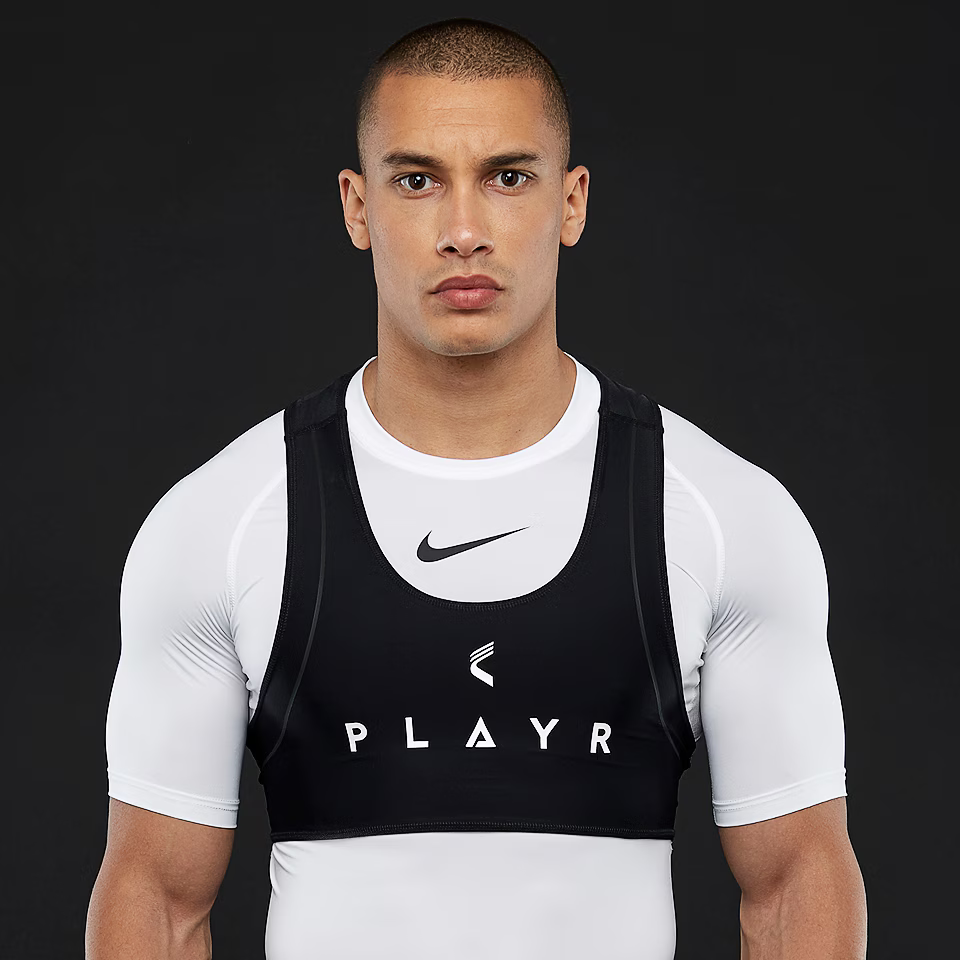
\includegraphics[width=0.3\linewidth]{img/peto.png}
    \caption[Peto deportivo de referencia]{Peto deportivo de referencia. Imagen obtenida de Pro:Direct Sport. Disponible en: \url{https://images.prodirectsport.com/ProductImages/Main/V3_1_Main_0289806.jpg}}
    \label{fig:peto}
\end{figure}

% LINK IMAGEN https://images.prodirectsport.com/ProductImages/Main/V3_1_Main_0289806.jpg


Las principales ventajas de este diseño eran principalmente la facilidad al momento de integrar los sensores, debido a que los circuitos no tendrían que ser tan pequeños. Además, algunas mediciones serían más sencillas de realizar, como las del sensor de ECG.

Sin embargo, existían complicaciones técnicas que nos limitaron a seguir pensando esta opción. La primera de ellas es que quizás sería muy complejo adaptar un circuito a un material más flexible y cómodo para el usuario, considerando que si se utilizan cables la posibilidad de aumentar el ruido entre los sensores y el microcontrolador eran muy altas. También, investigando en algunos de los posibles sensores que podíamos utilizar, algunos fueron diseñados para realizar mediciones en la zona de la muñeca. Por último, analizando desde un punto de vista higiénico, notamos que sería dificil permitir el lavado de la prenda sin generar daños a la circuitería.

\subsection{Dispositivo \textit{wearable} tipo \textit{smartband}}
Una de los requisitos de diseño implicaba la necesidad de utilizar una pantalla que mostrara los datos sensados, por lo que consideramos que una decisión de diseño fundamental para nuestro producto es que el usuario tuviera fácil acceso y visualización de los datos que el dispositivo mide. Es por ello que analizamos la opción de diseñar un dispositivo que se utilizara en la muñeca y pueda ser fácilmente manipulado por el usuario. La \rfigura{fig:smartband} presenta una \textit{smartband} comercial que sirvió como referencia para esta alternativa, mostrando el factor de forma compacto, la pantalla integrada y la correa ajustable que caracterizan a este tipo de dispositivos.

\begin{figure}[H]
    \centering
    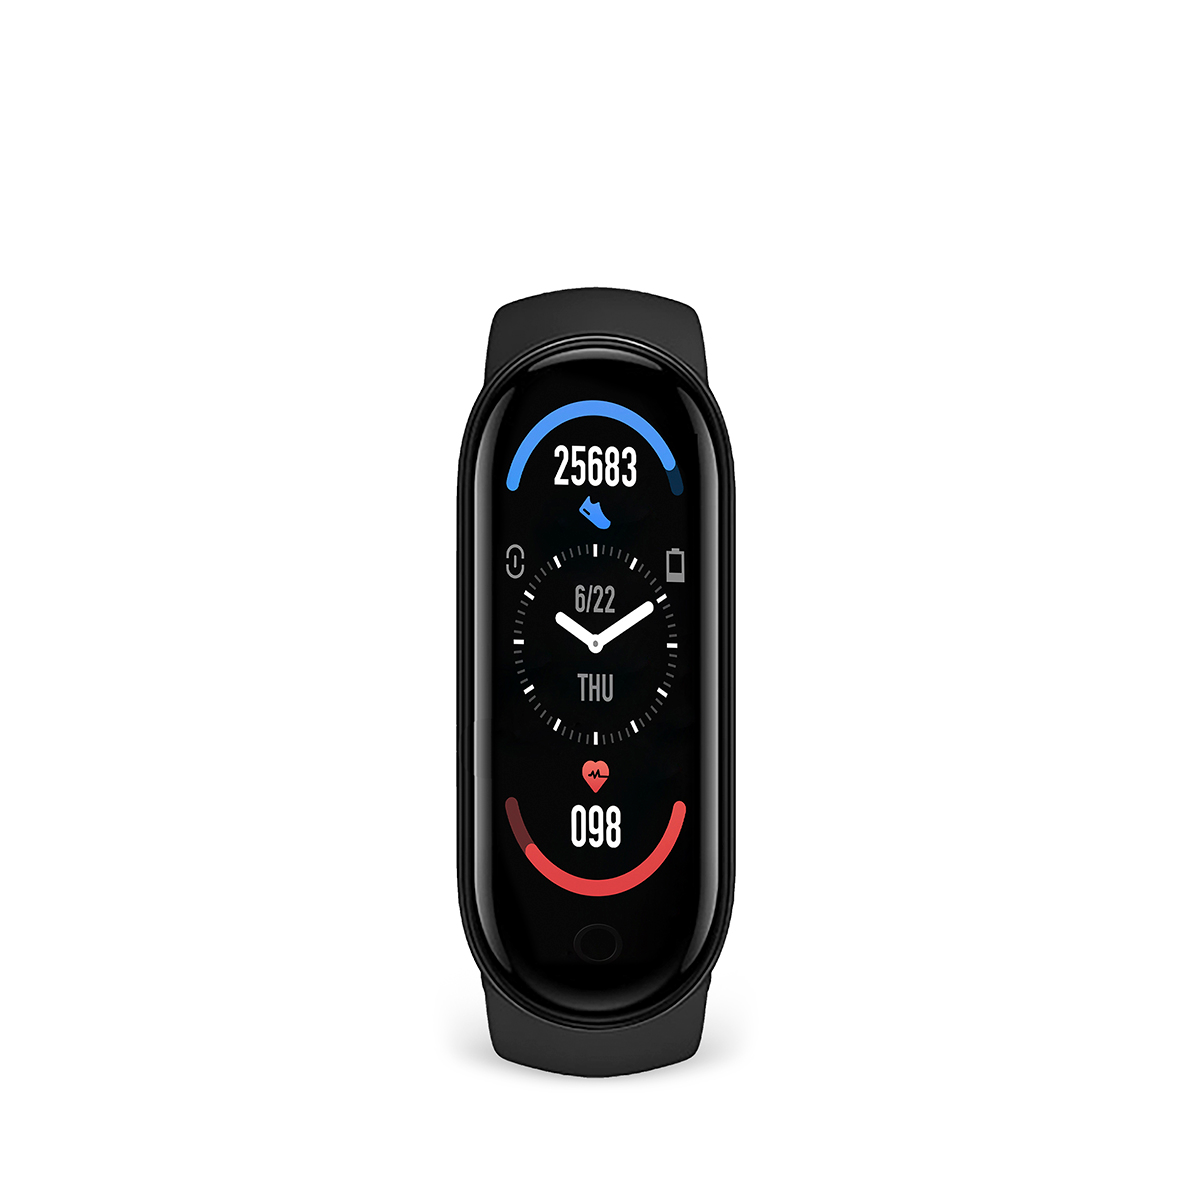
\includegraphics[width=0.3\linewidth]{img/smartband.png}
    \caption[\textit{Smartband} comercial de referencia]{\textit{Smartband} comercial de referencia (Prixton AT410). Disponible en: \url{https://prixton.com/product/smartband-at410/}}
    \label{fig:smartband}
\end{figure}

% LINK FOTO https://www.google.com/url?sa=t&source=web&rct=j&url=https%3A%2F%2Fprixton.com%2Fproduct%2Fsmartband-at410%2F&ved=0CBYQjRxqFwoTCKD8_PDUt5MDFQAAAAAdAAAAABAI&opi=89978449

El diseño del producto como \textit{smartband} tiene como ventaja que, al existir una gran variedad de dispositivos de la misma índole en el mercado, existe mucha documentación relacionada al diseño de estos dispositivos, incluyendo sensores adaptados para realizar mediciones en la zona de la muñeca dado que el grosor de la piel en esta zona es menor y permite un mejor monitoreo de las señales corporales como la saturación de oxígeno en sangre. Por otra parte, este dispositivo sería menos invasivo y más adaptable a distintos perfiles de usuarios, considerando que nuestro público objetivo puede variar significativamente su contextura física.

Más allá de las ventajas mencionadas anteriormente, existen distintos desafíos que deben ser tomados en cuenta para diesñar este tipo de dispositivos. La primera consideración es que el producto debe ser pequeño para no generar incomodidades al usuario, esto es una limitación a nivel de diseño y de ingeniería, pues se debe considerar que la batería que tendrá el dispositivo será pequeña y no podemos considerar componentes que consuman mucha corriente para maximizar la duración de la batería, considerando que debemos incluir un modelo de \textit{Machine Learning} dentro o fuera del dispositivo, lo cual es una tarea exigente que puede demandar mucha memoria del microcontrolador si se realiza interna o mucho consumo energético si se envían muchos paquetes de forma inalámbrica a un servidor para su posterior análisis. Siguiendo la línea de la comodidad, se vuelve fundamental la necesidad de miniaturizar el dispositivo, principalmente los componentes utilizados para el funcionamiento óptimo de los sensores, utilizando idealmente componentes SMD, lo cual puede ser difícil considerando que el laboratorio de trabajo no tiene instrumentos ni herramientas óptimos para realizar PCB que utilicen estos componentes.


\section{Propuesta de diseño}

En base al análisis de las opciones anteriores, se optó por el desarrollo de un \textit{wearable} tipo smartwatch debido a la amplia disponibilidad de componentes adaptados para biometría periférica y la facilidad de interacción directa con el usuario, así como no tener que lidiar con los largos recorridos de las señales de estar situadas muy lejos entre sí físicamente.

El producto a desarrollar es \textbf{SupaClock}, un \textit{wearable} enfocado en el monitoreo biométrico y de actividad física. El entregable principal del proyecto consistirá en un dispositivo compacto, cómodo y completamente funcional. La primera iteración contendrá todos los subsistemas y sensores sobre una PCB básica. Luego de verificar el funcionamiento general, se migrará a una PCB personalizada con los circuitos de los sensores, alimentación, microcontrolador y periféricos, así como una carcasa hecha a medida. El sistema será orquestado inicialmente por el microcontrolador ESP32 C3 \citep{esp32c3_ds}, dependiendo de su desempeño en etapas iniciales de prueba, se considera migrar hacia el ESP32 S3 \citep{esp32s3_ds}, que tiene varias mejoras significativas, a costa de un mayor consumo energético. Para gestionar el lado de software, se dispondrá del sistema operativo FreeRTOS \citep{freertos_ref}.

Como objetivo extendido (\textit{bonus}), una vez validada la arquitectura principal, se diseñará una versión "Pro". Esta consistirá en una placa PCB miniaturizada de alta densidad, acercándose a un factor de forma de \textit{smartwatch} comercial. De manera complementaria, el ecosistema se expandirá con una aplicación Android que recibirá los datos vía Bluetooth Low Energy (BLE) y los almacenará de forma persistente en una base de datos en la nube (como Firebase), permitiendo un análisis histórico y avanzado de las métricas del usuario.

Para satisfacer los requerimientos técnicos del proyecto, la propuesta de diseño integra múltiples subsistemas. En primer lugar, la adquisición de señales biológicas se realiza mediante el sensor MAX30102 \citep{max30102_ds} para fotopletismografía (SpO2/HR) y el MAX30205 \citep{max30205_ds} para la temperatura corporal, exigiéndose un diseño mecánico que garantice un contacto dérmico directo, constante y cómodo en la muñeca. Complementariamente, se implementa un sistema de electrocardiografía monocanal basado en el circuito AD8232 \citep{ad8232_ds}, el cual utiliza un arreglo de tres electrodos de contacto seco (pernos M3) distribuidos en el dispositivo; esto permite medir la Derivación I del corazón mediante una interacción sencilla, requiriendo únicamente que el usuario haga contacto con la mano opuesta sobre un perno situado en la carcasa. En cuanto al monitoreo de la actividad, se integra un acelerómetro y giroscopio (BMI160) \citep{bmi160_ds} para la captura de telemetría inercial en 6 ejes, datos que alimentarán un modelo de Machine Learning capaz de distinguir estados físicos como \textit{caminar, correr, reposo}, o detectar situaciones de \textit{emergencia/caída}. Finalmente, la retroalimentación al usuario se resuelve mediante un despliegue gráfico local, incorporando una pantalla LCD a color \citep{st7789_ds} para renderizar una interfaz fluida, atractiva y prolija, capaz de mostrar métricas numéricas y formas de onda de manera completamente autónoma y sin depender del teléfono móvil.

\section{Análisis de requerimientos}
\subsection{Dispositivo compacto y cómodo}
Al escoger un \textit{wearable}, debemos diseñar un dispositivo que no imposibilite el uso de la muñeca, por lo que no puede superar los 80 mm de largo ni 50 mm de ancho.  A su vez, la altura del dispositivo puede generar incomodidad, por lo que debemos realizar un diseño que no supere los 30 mm de altura. Por otra parte, el peso es un factor importante, por lo que nuestro dispositivo no puede pesar más de 150 g.

Dada la naturaleza de algunos sensores, es necesario que algunos de estos deban tener contacto directo con la piel del usuario, por lo que es fundamental que estos se encuentren correctamente protegidos y aislados. Considerando los implementos del laboratorio, realizaremos una carcasa impresa en 3D que albergue todos los componentes en su interior, y que permita una interacción segura entre los sensores y el usuario.


\subsection{Energización y autonomía}
El dispositivo no puede estar energizado a una fuente de poder para su uso cotidiano, por lo que es fundamental el uso de baterías para alimentar al mismo. Para garantizar un uso óptimo y seguro de la misma, se debe incluir un BMS en el diseño. A su vez, es necesario incluir un circuito \textit{battery fuel gauge}, el integrado MAX17043 se encarga de informar mediante I2C el nivel de batería al usuario.

Para ser un dispositivo a la altura de la competencia, es necesario que la batería tenga una duración mínima de 12 horas, por lo que es necesario optimizar los consumos de energía del microcontrolador y los sensores del dispositivo.

\subsection{Mediciones requeridas}

Para cumplir íntegramente con las especificaciones del proyecto, el hardware del dispositivo debe ser capaz de adquirir, acondicionar y digitalizar cinco variables biométricas y cinemáticas fundamentales, garantizando la entrega de señales limpias para su posterior procesamiento:

\begin{itemize}
    \item \textbf{Temperatura corporal superficial:} Capturada de manera periódica mediante el sensor de grado clínico MAX30205, el cual requiere un diseño mecánico que asegure contacto térmico directo con la piel del usuario.
    \item \textbf{Frecuencia cardíaca y Saturación de oxígeno (SpO2):} Ambas métricas serán estimadas mediante fotopletismografía (PPG) de reflectancia, utilizando el módulo óptico MAX30102 ubicado en la base del dispositivo.
    \item \textbf{Aceleración:} La captura del movimiento lineal espacial (necesaria tanto para el podómetro como para el modelo de clasificación) se realizará mediante la Unidad de Medición Inercial (IMU) BMI160.
    \item \textbf{Electrocardiograma (ECG):} Se requiere la adquisición de la actividad eléctrica del corazón. Esta función estará destinada de manera exclusiva a \textbf{mediciones puntuales en estado de reposo}. Para ello, se utilizará el módulo de instrumentación analógica AD8232 acoplado a un arreglo de tres electrodos de contacto seco (pernos M3), requiriendo que el usuario cierre el circuito bioeléctrico mediante contacto bimanual. Estos datos serán procesados inicialmente en el microcontrolador, para luego enviarse vía bluetooth al teléfono, el cual subirá los datos al servidor que guardará el perfil del usuario, junto con hacer un análisis más profundo de las métricas diarias.
\end{itemize}

\subsection{Procesamiento algorítmico y Machine Learning}
El dispositivo no solo actúa como un recolector de datos, sino que debe procesarlos localmente, cumpliendo con los siguientes requerimientos algorítmicos:
\begin{itemize}
    \item \textbf{Contador de pasos algorítmico:} Dadas las restricciones del proyecto de no utilizar módulos comerciales pre-programados, se desarrollará un algoritmo propietario en C++. Este operará calculando la magnitud del vector tridimensional de aceleración ($|a| = \sqrt{a_x^2 + a_y^2 + a_z^2}$). A esta señal cruda se le aplicará un filtro pasabajos (como una media móvil) para atenuar vibraciones de alta frecuencia, seguido de un algoritmo de detección de picos con un umbral (\textit{threshold}) adaptativo para contabilizar el paso. Este contador contará con la funcionalidad de ser reseteado a cero a voluntad del usuario navegando por los menús de la interfaz gráfica local del \textit{smartwatch}.

    \item \textbf{Clasificación de actividades (4 estados):} Se requiere implementar un modelo de clasificación capaz de predecir cuatro estados físicos y situaciones de riesgo: \textit{reposo}, \textit{caminar}, \textit{correr} y detección de \textit{caída/emergencia}. Este último estado es crítico para otorgar un valor añadido a la seguridad del usuario.

    \item \textbf{Justificación de la arquitectura Edge AI:} Se ha decidido implementar el modelo de Inteligencia Artificial directamente en el microcontrolador (\textit{Edge Computing/TinyML}) en lugar de procesarlo en la nube. Esta decisión se justifica por tres factores clave: minimiza la latencia (aspecto crítico para reportar una caída en tiempo real), reduce drásticamente el consumo energético al evitar la transmisión constante de telemetría cruda por la antena Bluetooth, y garantiza la privacidad de los movimientos del usuario. Para el flujo de trabajo, se evaluará el uso de la plataforma \textbf{Edge Impulse} \citep{edge_impulse} y \textbf{TensorFlow Lite for Microcontrollers} \citep{tflite_micro}, herramientas que permiten entrenar la red neuronal y compilarla en una librería en C++ altamente optimizada para las instrucciones vectoriales del ESP32-S3 o código simple cuantizado para ESP32-C3.
\end{itemize}

\subsection{Algoritmos de Procesamiento de Señales (ECG)}
Para la estimación precisa de la frecuencia cardíaca a partir de la señal analógica del módulo AD8232, se implementará el algoritmo estándar de \textbf{Pan-Tompkins} \citep{pan_tompkins}. Para no sobrecargar el microcontrolador y conservar batería, este procesamiento se ejecutará de manera asíncrona en la nube una vez recibida la trama de datos:

\begin{enumerate}
    \item \textbf{Filtrado Digital Pasabanda:} Se aplicará un filtro digital para atenuar el ruido de alta frecuencia (interferencia de la red eléctrica) y eliminar la deriva de la línea base causada por la respiración del usuario.
    \item \textbf{Procesamiento Morfológico:} La señal filtrada pasará por un filtro derivativo y una función de cuadratura para resaltar exclusivamente la pendiente aguda del complejo QRS del corazón.
    \item \textbf{Detección de Picos R:} Se utilizará una integración de ventana móvil con umbrales adaptativos (\textit{adaptive thresholding}) para identificar con precisión el tiempo exacto de cada latido.
    \item \textbf{Cálculo de Métricas:} A partir de la distancia temporal entre picos consecutivos (intervalos R-R), el sistema calculará la Frecuencia Cardíaca promedio (BPM) y devolverá el valor a la aplicación móvil para su visualización.
\end{enumerate}


\subsection{Interfaz gráfica y navegación}
Para asegurar una interacción intuitiva y cumplir con los requerimientos de visualización local sin depender exclusivamente del teléfono móvil, el dispositivo integrará una pantalla LCD rectangular a color de 1.69 pulgadas. El sistema de navegación físico constará de tres botones pulsadores (Arriba, Abajo y Seleccionar/Acción) ubicados en el costado derecho de la carcasa, garantizando una operación intuitiva y fácil, incluso durante la actividad física.

La interfaz gráfica de usuario (GUI) se ha diseñado maximizando el contraste mediante un fondo negro e íconos de colores vibrantes para una rápida lectura. El sistema se estructurará lógicamente en cuatro vistas principales, las cuales se pueden apreciar en la \rfigura{fig:pantallas}:

\begin{figure}[H]
    \centering
    \includegraphics[width=1.0\textwidth]{img/pantallas.png} % Asegúrate de que la ruta coincida con tu carpeta
    \caption{Diseño preliminar de las interfaces gráficas del dispositivo.}
    \label{fig:pantallas}
\end{figure}

\begin{enumerate}
    \item \textbf{Pantalla Principal (Dashboard):} Actuará como la carátula central (\textit{watchface}). Concentra la información de uso continuo exigida por los requerimientos: la hora actual, el contador de pasos, el nivel porcentual de batería, la frecuencia cardíaca y la actividad física predicha por el modelo de IA en ese instante.
    \item \textbf{Biometría General:} Un panel dedicado a mostrar las lecturas de los sensores periféricos, desplegando la frecuencia cardíaca, el porcentaje de saturación de oxígeno (SpO2) y la temperatura corporal superficial, además de indicar el estado operativo de los sensores.
    \item \textbf{Modo ECG:} Interfaz interactiva orientada exclusivamente a la toma del electrocardiograma en estado de reposo. Guiará al usuario mediante instrucciones visuales para que cierre el circuito bimanual tocando los electrodos. Adicionalmente, mostrará una cuenta regresiva del progreso y dibujará (se está evaluando la posibilidad) la forma de onda cardíaca en tiempo rea.
    \item \textbf{Menú del Sistema:} Interfaz de configuración general que albergará opciones avanzadas. Aquí se incluirá la función de reiniciar a cero el contador de pasos, activar el modo de emparejamiento Bluetooth (BLE) para la sincronización de datos (\textit{Data Logger}) con la aplicación móvil/PC y gestionar el apagado del equipo.
\end{enumerate}
\section{Elección de componentes y justificación}

El componente más importante de nuestro \textit{wearable} es el microcontrolador, ya que actúa como el cerebro del sistema: gobierna todos los periféricos, ejecuta los algoritmos de procesamiento de señales, corre el modelo de \textit{Machine Learning} y gestiona las comunicaciones inalámbricas. Una elección inadecuada en esta etapa comprometería la autonomía energética, la capacidad de procesamiento y la viabilidad de futuras expansiones del producto.

A continuación se presenta una tabla comparativa de las distintas opciones analizadas como MCU del \textit{wearable}. Es importante aclarar que los tamaños utilizados para la columna de dimensiones están referidos a módulos que tienen integrados los microcontroladores mencionados.
\begin{table}[H]
    \centering
    \renewcommand{\arraystretch}{1.3}
    \begin{tabular}{|L{2.5 cm}|L{2.5 cm}|L{2.5 cm}|L{2 cm}|L{2 cm}|L{2 cm}|L{1.7 cm}|}
        \hline
        \textbf{MCU}                                                                                                           & \textbf{Arch y Freq}                 & \textbf{Math Process (DSP/ML)}                                                                               & \textbf{Connect}                                  & \textbf{Power Consumption}                                                              & \textbf{Size/ Integration}                                 & \textbf{PinOut GPIO} \\ \hline


        %https://es.aliexpress.com/item/1005006391993583.html?spm=oneshop.outseo.search.6.301c1kuM1kuM9D&skuId=12000037002719702&pdp_ext_f=%7B%22sku_id%22%3A%2212000037002719702%22%7D&gatewayAdapt=glo2esp#nav-specification
        %https://www.mouser.cl/datasheet/3/1574/1/esp32-c3-mini-1_datasheet_en.pdf
        \textbf{ESP32-C3 SUPER MINI (Seleccionado)} \citep{esp32c3_ds}                                                         & RISC-V 32-bit de un núcleo (160 MHz) & \textbf{Por software.} No posee FPU (hardware), los cálculos de ML y filtros requerirán más ciclos de reloj. & WiFi 4 y Bluetooth 5 (LE)                         & \textbf{Medio.} Requiere diseño cuidadoso de Deep Sleep.                                & 22.5 mm x 18 mm                                            & 13                   \\ \hline

        % https://documentation.espressif.com/esp32-s3_datasheet_en.pdf
        %https://es.aliexpress.com/item/1005010580012002.html?spm=a2g0o.productlist.main.1.1e2bNmbgNmbgOT&algo_pvid=30dd6bc5-45f1-4c71-a3b7-0bb2b845a91d&algo_exp_id=30dd6bc5-45f1-4c71-a3b7-0bb2b845a91d-0&pdp_ext_f=%7B%22order%22%3A%221527%22%2C%22eval%22%3A%221%22%2C%22fromPage%22%3A%22search%22%7D&pdp_npi=6%40dis%21CLP%213861%213370%21%21%2128.23%2124.64%21%4021033d1217744802500498130e2adc%2112000052880779511%21sea%21CL%210%21ABX%211%210%21n_tag%3A-29910%3Bd%3A8ad082ff%3Bm03_new_user%3A-29895%3BpisId%3A5000000197837106&curPageLogUid=sU0GknIeFm7q&utparam-url=scene%3Asearch%7Cquery_from%3A%7Cx_object_id%3A1005010580012002%7C_p_origin_prod%3A
        \textbf{ESP32-S3 (Seleccionado)} \citep{esp32s3_ds}                                                                    & Xtensa 32-bit Dual-Core (240 MHz)    & \textbf{Sobresaliente.} Posee instrucciones vectoriales para acelerar redes neuronales.                      & WiFi 4 y Bluetooth 5 (LE)                         & \textbf{Alto.} Consumo peak de 340 mA transmitiendo por Wifi 2.4 GHz, 1 Mbps y 21 dBm . & Muy bueno, pero requiere un área de PCB ligeramente mayor. & 27                   \\ \hline


        \textbf{NRF52840} \citep{nrf52840_ds}                                                                                  & ARM Cortex-M4F (64 MHz)              & \textbf{Excelente.} Posee FPU por hardware, ideal para el filtrado del ECG y ML de bajo consumo.             & Solo Bluetooth 5 (LE) y otros. \textbf{Sin WiFi.} & \textbf{Ultra Bajo.} Perfecto para wearables de alta autonomía.                         & Excelente, existen módulos SMD diminutos.                  & 11                   \\ \hline

        \textbf{STM32WB55} \citep{stm32wb55_ds}                                                                                &
        Dual-Core: ARM Cortex-M4 (64 MHz) para aplicación y Cortex-M0+ (32 MHz) dedicado a radio.                              &
        \textbf{Excelente.} Posee FPU por hardware y soporte nativo optimizado para ML                                         &
        Bluetooth 5 (LE) y 802.15.4 (Zigbee/Thread). \textbf{Sin WiFi.}                                                        &
        \textbf{Ultra Bajo.} El procesador de radio independiente permite ahorrar mucha batería durante las transmisiones.     &
        \textbf{Muy bueno.} Empaquetados muy pequeños, pero requiere un diseño de antena RF si no se compra en formato módulo. &
        22                                                                                                                                                                                                                                                                                                                                                                                                                                                                                                             \\ \hline
    \end{tabular}
    \caption{Comparación de Opciones de Microcontroladores (MCU)}
    \label{tab:mcu_comparison}
\end{table}

La decisión de utilizar la familia de microcontroladores de Espressif (\textbf{ESP32-C3} y \textbf{ESP32-S3}) se fundamenta en su \textbf{facilidad de desarrollo} y la \textbf{vasta cantidad de documentación} y herramientas disponibles que el equipo ya domina. Esto permite acelerar significativamente la fase de prototipado. Adicionalmente, la compatibilidad en el ecosistema de Espressif ofrece una tremenda flexibilidad: el proyecto iniciará utilizando el \textbf{ESP32-C3} debido a su bajo costo y menor consumo energético, con la \textbf{posibilidad de migrar fácilmente al ESP32-S3} sin mayores cambios en el código base, en caso de que el modelo de \textit{Machine Learning} y los algoritmos de procesamiento exijan una \textbf{mayor potencia de cómputo}.

\begin{table}[H]
    \centering
    \renewcommand{\arraystretch}{1.3}
    \begin{tabular}{|L{2.5cm}|L{2.0cm}|L{2.5cm}|L{2.5cm}|L{3.5cm}|}
        \hline
        \textbf{Sensor (Fabricante)}                             & \textbf{Interfaz} & \textbf{Resolución}   & \textbf{Consumo (Modo Activo)} & \textbf{Ventajas / Desventajas}                                                                                           \\ \hline
        \textbf{BMI160 (Bosch) - Seleccionado} \citep{bmi160_ds} & I2C / SPI         & 16 bits (Acel + Giro) & $\sim$900 $\mu$A               & \textbf{Ventaja:} Excelente eficiencia y buffer FIFO grande (1024 bytes). Ideal para Edge ML.                             \\ \hline
        \textbf{MPU6050 (InvenSense)} \citep{mpu6050_ds}         & I2C               & 16 bits (Acel + Giro) & $\sim$3900 $\mu$A (3.9 mA)     & \textbf{Desventaja:} Consumo de energía excesivamente alto para un wearable. Tecnología antigua (Legacy).                 \\ \hline
        \textbf{LSM6DS3 (STMicro)} \citep{lsm6ds3_ds}            & I2C / SPI         & 16 bits (Acel + Giro) & $\sim$1250 $\mu$A              & \textbf{Ventaja:} Muy bajo consumo y contador de pasos por hardware integrado (aunque el proyecto exige software propio). \\ \hline
    \end{tabular}
    \caption{Comparación de Sensores Inerciales (IMU) para Detección de Actividad}
    \label{tab:imu_comparison}
\end{table}

Para la detección de movimiento continuo (podómetro y clasificación de Machine Learning), la \rtabla{tab:imu_comparison} evidencia que el BMI160 es la opción idónea al combinar un consumo por debajo de 1 mA y un amplio buffer FIFO (que desacopla el trabajo de lectura continua del microcontrolador), descartando alternativas de tecnología más antigua y alto perfil energético como el MPU6050.


\begin{table}[H]
    \centering
    \renewcommand{\arraystretch}{1.3}
    \begin{tabular}{|L{2.5cm}|L{2.0cm}|L{2.5cm}|L{2.5cm}|L{3.5cm}|}
        \hline
        \textbf{Sensor (Fabricante)}                                 & \textbf{Interfaz} & \textbf{Resolución ADC} & \textbf{Consumo Promedio}  & \textbf{Ventajas / Desventajas}                                                                                                      \\ \hline
        \textbf{MAX30102 (Maxim) - Seleccionado} \citep{max30102_ds} & I2C               & 18 bits                 & $\sim$600 $\mu$A           & \textbf{Ventaja:} Integra LEDs y fotodetector. Alta resolución y cristal protector que facilita la limpieza en contacto con la piel. \\ \hline
        \textbf{MAX30100 (Maxim)} \citep{max30100_ds}                & I2C               & 16 bits                 & $\sim$1200 $\mu$A          & \textbf{Desventaja:} Menor resolución, mayor consumo y conocido por problemas de compatibilidad de voltajes en módulos comerciales.  \\ \hline
        \textbf{MAX86141 (Maxim)} \citep{max86141_ds}                & SPI               & 19 bits                 & Ultra bajo ($<$100 $\mu$A) & \textbf{Desventaja:} Requiere LEDs externos y diseño de hardware sumamente complejo. Excede el alcance de un prototipo inicial.      \\ \hline
    \end{tabular}
    \caption{Comparación de Sensores Ópticos (PPG) para HR y SpO2}
    \label{tab:ppg_comparison}
\end{table}

Por el lado de la métrica cardíaca y de oxigenación, en la \rtabla{tab:ppg_comparison} se analiza el abanico de fotopletismógrafos comerciales. El MAX30102 se consagra como nuestra elección principal por su excelente relación de facilidad de uso e integración, ya que compila ópticas de alta resolución en un encapsulado que incluye vidrio protector ideal para el contacto epitelial constante en la muñeca, superando las limitaciones de versiones antiguas como el MAX30100.

\begin{table}[H]
    \centering
    \renewcommand{\arraystretch}{1.3}
    \begin{tabular}{|L{2.5cm}|L{2.0cm}|L{2.5cm}|L{2.5cm}|L{3.5cm}|}
        \hline
        \textbf{Sensor (Fabricante)}                                 & \textbf{Interfaz} & \textbf{Precisión (Rango Clínico)}            & \textbf{Consumo Activo} & \textbf{Ventajas / Desventajas}                                                                                                   \\ \hline
        \textbf{MAX30205 (Maxim) - Seleccionado} \citep{max30205_ds} & I2C               & $\pm$0.1$^\circ$C (37$^\circ$C a 39$^\circ$C) & $\sim$600 $\mu$A        & \textbf{Ventaja:} Precisión de grado clínico específica para piel humana. Fácil integración en bus I2C.                           \\ \hline
        \textbf{MLX90614 (Melexis)} \citep{mlx90614_ds}              & I2C / PWM         & $\pm$0.2$^\circ$C                             & $\sim$1.5 mA            & \textbf{Desventaja:} Medición infrarroja sin contacto. Es muy voluminoso (empaque TO-39) e inviable para un diseño ultracompacto. \\ \hline
        \textbf{DS18B20 (Maxim)} \citep{ds18b20_ds}                  & 1-Wire            & $\pm$0.5$^\circ$C                             & $\sim$1 mA              & \textbf{Desventaja:} Precisión insuficiente para uso biomédico y el protocolo 1-Wire consume más recursos de software que el I2C. \\ \hline
    \end{tabular}
    \caption{Comparación de Sensores de Temperatura para Aplicaciones Médicas/Wearables}
    \label{tab:temp_comparison}
\end{table}

La medición de fiebre o estrés térmico requiere alta fidelidad; como describe la \rtabla{tab:temp_comparison}, descartamos medidores de propósito general (DS18B20) o módulos infrarrojos muy abultados (MLX90614, propio de termómetros de pistola). En contraste, el MAX30205 proporciona precisión con certificación clínica ($\pm$0.1$^\circ$C en rango humano) mediante simple contacto superficial con la piel.

\begin{table}[H]
    \centering
    \renewcommand{\arraystretch}{1.3}
    \begin{tabular}{|L{2.5cm}|L{2.5cm}|L{2.5cm}|L{2.0cm}|L{3.5cm}|}
        \hline
        \textbf{IC de Carga (Fabricante)}                        & \textbf{Topología}             & \textbf{Protección Integrada}   & \textbf{Corriente de Carga} & \textbf{Ventajas / Desventajas}                                                                                                                               \\ \hline
        \textbf{TP4056 + DW01A - Seleccionado} \citep{tp4056_ds} & Cargador Lineal LDO            & Requiere IC externo (DW01A)     & Hasta 1A (Ajustable)        & \textbf{Ventaja:} Costo extremadamente bajo, circuito comprobado y fácil de soldar a mano. Ideal para el prototipo.                                           \\ \hline
        \textbf{BQ24075 (Texas Instruments)} \citep{bq24075_ds}  & Cargador Lineal con Power-Path & Sí (Sobretensión y Temperatura) & Hasta 1.5A                  & \textbf{Desventaja:} Costoso y empaquetado QFN difícil de ensamblar. \textbf{Ventaja:} Permite usar el dispositivo mientras se carga sin estresar la batería. \\ \hline
        \textbf{MCP73831 (Microchip)} \citep{mcp73831_ds}        & Cargador Lineal                & No (Solo gestión térmica)       & Hasta 500 mA                & \textbf{Desventaja:} Aunque es diminuto (SOT-23), carece de protección contra sobredescarga, obligando a añadir más circuitería.                              \\ \hline
    \end{tabular}
    \caption{Comparación de Circuitos Integrados para Carga y Protección (BMS)}
    \label{tab:bms_comparison}
\end{table}

Respecto a la fuente de poder, se seleccionó una \textbf{batería de polímero de litio (LiPo) de 3.7V}. Según el análisis y perfilado de consumo de los diferentes periféricos operando bajo \textit{FreeRTOS}, hemos estimado un requerimiento energético en torno a los \textbf{350 mAh} para asegurar una autonomía funcional de aproximadamente \textbf{un día completo}, manteniendo al mismo tiempo un factor de forma delgado y liviano fundamental para un dispositivo tipo pulsera. Para la gestión térmica y energética de dicha celda, la \rtabla{tab:bms_comparison} resume el análisis del subsistema de carga (BMS). La combinación de los integrados genéricos TP4056 y el circuito de protección DW01A es ideal para el primer prototipo. Este módulo se adquiere fácilmente soldado en placa base con puerto Type-C integrado por un valor bajo, superando las barreras de soldadura que ofrecen QFNs como el BQ24075.

\begin{table}[H]
    \centering
    \renewcommand{\arraystretch}{1.3}
    \begin{tabular}{|L{2.5cm}|L{2.5cm}|L{2.5cm}|L{2.0cm}|L{3.5cm}|}
        \hline
        \textbf{Componente (Fabricante)}                             & \textbf{Método de Medición}        & \textbf{Hardware Externo} & \textbf{Consumo Promedio}    & \textbf{Ventajas / Desventajas}                                                                                                           \\ \hline
        \textbf{MAX17043 (Maxim) - Seleccionado} \citep{max17043_ds} & ModelGauge (Basado en voltaje)     & Ninguno                   & $\sim$50 $\mu$A              & \textbf{Ventaja:} Estima el estado de carga (SOC) sin resistencia de sensado (shunt), ahorrando valioso espacio en la PCB.                \\ \hline
        \textbf{BQ27441-G1 (Texas Instruments)} \citep{bq27441_ds}   & Impedance Track (Coulomb Counting) & Resistencia Shunt externa & $\sim$93 $\mu$A              & \textbf{Desventaja:} Mayor precisión, pero requiere ruteo crítico de la resistencia shunt y configuración compleja del perfil de batería. \\ \hline
        \textbf{Lectura directa por ADC (ESP32)}                     & Divisor de voltaje resistivo       & 2 Resistencias            & Variable (Corriente de fuga) & \textbf{Desventaja:} El ADC del ESP32 no es lineal. Desperdicia batería por el divisor de tensión y es muy impreciso.                     \\ \hline
    \end{tabular}
    \caption{Comparación de Monitores de Batería (Fuel Gauges)}
    \label{tab:fuelgauge_comparison}
\end{table}

Representar el \textit{State of Charge} (nivel de batería en la pantalla de la muñeca) sin dañar la autonomía general requiere un integrado especializado. Tal como indica la \rtabla{tab:fuelgauge_comparison}, la decisión decantó por el MAX17043 ya que utiliza el algoritmo patentado \textit{ModelGauge} sobre el voltaje crudo (sin utilizar derivadores shunt externos o puentes resistivos analógicos), ahorrando considerable consumo estático en la placa.

\begin{table}[H]
    \centering
    \renewcommand{\arraystretch}{1.3}
    \begin{tabular}{|L{2.5cm}|L{2.0cm}|L{2.5cm}|L{2.5cm}|L{3.5cm}|}
        \hline
        \textbf{Regulador LDO}                                     & \textbf{Corriente Máxima} & \textbf{Voltaje de Caída (Dropout)} & \textbf{Corriente Quiescente ($I_Q$)} & \textbf{Ventajas / Desventajas}                                                                                                                        \\ \hline
        \textbf{ME6211 / AP2112K - Seleccionado} \citep{me6211_ds} & $\sim$500 mA              & Ultra bajo ($\sim$100 mV a 100 mA)  & $\sim$55 $\mu$A                       & \textbf{Ventaja:} Excelente balance entre tamaño (SOT-23-5), eficiencia cuando la batería baja de 3.6V y capacidad de corriente para el WiFi.          \\ \hline
        \textbf{AMS1117-3.3} \citep{ams1117_ds}                    & 1 A                       & Muy alto ($\sim$1.1 V)              & $\sim$5 mA (5000 $\mu$A)              & \textbf{Desventaja:} Pésima elección para baterías. Su alto dropout cortaría el ESP32 incluso cuando la batería esté al 50\%. Drena energía en reposo. \\ \hline
        \textbf{TPS7A02 (Texas Instruments)} \citep{tps7a02_ds}    & 200 mA                    & Bajo ($\sim$140 mV)                 & Nano-poder (25 nA)                    & \textbf{Desventaja:} Corriente máxima insuficiente para los picos de transmisión WiFi del ESP32-C3 (que superan los 300 mA).                           \\ \hline
    \end{tabular}
    \caption{Comparación de Reguladores de Voltaje LDO (3.3V) para Fase 2}
    \label{tab:ldo_comparison}
\end{table}

Traducir los voltajes inestables de la batería de litio (4.2V a 3.0V) a los estables 3.3V que demanda el microcontrolador debe hacerse con máxima eficiencia térmica y con el mínimo dropout posible (Voltaje de caída extra). La \rtabla{tab:ldo_comparison} deja en evidencia que reguladores comunes (como el AMS1117) son pésimos para baterías móviles; por ello, elegimos el ME6211, el cual puede entregar ráfagas de alta corriente sin bloquearse cuando la celda baje de 3.6V.


\begin{table}[H]
    \centering
    \renewcommand{\arraystretch}{1.3}
    \begin{tabular}{|L{3.4cm}|L{1.8cm}|L{2.6cm}|L{2.8cm}|L{4.2cm}|}
        \hline
        \textbf{Tecnología (Controlador)}                               & \textbf{Interfaz} & \textbf{Color y Resolución} & \textbf{Consumo Estimado}                   & \textbf{Ventajas / Desventajas}                                                                                                                                   \\ \hline
        \textbf{IPS LCD 1.3" (ST7789) - Seleccionado} \citep{st7789_ds} & SPI               & RGB (240x240)               & Medio ($\sim$20-40 mA con retroiluminación) & \textbf{Ventaja:} Excelente densidad de píxeles, colores vibrantes para gráficas (ECG) y la interfaz SPI maneja la tasa de refresco sin cuellos de botella.       \\ \hline
        \textbf{OLED 0.96" (SSD1306)} \citep{ssd1306_ds}                & I2C / SPI         & Monocromo (128x64)          & Bajo-Medio ($\sim$10-20 mA)                 & \textbf{Desventaja:} Menor resolución y tamaño. Difícil visualizar 4 señales simultáneas y la predicción de Machine Learning de forma legible.                    \\ \hline
        \textbf{Memory LCD (Sharp)} \citep{sharpmem_ds}                 & SPI               & Monocromo (Alto contraste)  & Ultra bajo ($\sim$10 $\mu$A)                & \textbf{Desventaja:} Muy costosa y sin retroiluminación (ilegible en la oscuridad). Excelente para autonomía extrema, pero no justifica el costo en este alcance. \\ \hline
    \end{tabular}
    \caption{Comparación de Tecnologías de Pantalla para Interfaz de Usuario}
    \label{tab:display_comparison}
\end{table}

Finalmente, dotar al sistema de una cara visual local y dinámica decanta en la elección del controlador de pantalla ST7789 (\rtabla{tab:display_comparison}). Al descartar opciones monocromáticas limitadas o extremadamente costosas, la pantalla IPS permite un pintado en alta resolución que es ideal para dibujar los vectores del Electrocardiograma (ECG) en vivo, junto a una paleta de colores vibrantes para un entorno de usuario premium.

% ==========================================
% 2. DIAGRAMA DE BLOQUES
% ==========================================
\section{Diagrama de bloques}

\subsection{Diagrama de bloques de alto nivel }

Para la implementación de la propuesta, se planteó el diagrama de bloques de la \rfigura{fig:bloques}, el cual presenta una vista integral de todos los subsistemas del proyecto SupaClock y sus interacciones. El diagrama abarca desde la adquisición de señales biométricas en el dispositivo hasta el almacenamiento y análisis de datos en la nube, pasando por la aplicación móvil que actúa como enlace entre ambos dominios. Los colores de las cajas y las conexiones permiten identificar rápidamente cada dominio funcional, tal como se detalla en la leyenda incluida en la parte inferior del diagrama.

\shorthandoff{>}\shorthandoff{<}
\begin{figure}[H]
    \centering
    \resizebox{\textwidth}{!}{%
        \begin{tikzpicture}[
                node distance=0.8cm and 1.2cm,
                % Estilos de bloques
                userblock/.style={rectangle, rounded corners, draw=black, thick, fill=teal!15, text width=2.8cm, align=center, minimum height=1cm, font=\footnotesize},
                energyblock/.style={rectangle, rounded corners, draw=black, thick, fill=yellow!20, text width=2.5cm, align=center, minimum height=1cm, font=\footnotesize},
                sensorblock/.style={rectangle, rounded corners, draw=black, thick, fill=green!15, text width=2.5cm, align=center, minimum height=1cm, font=\footnotesize},
                mcublock/.style={rectangle, rounded corners, draw=black, thick, fill=blue!15, text width=3cm, align=center, minimum height=1.2cm, font=\footnotesize},
                ifaceblock/.style={rectangle, rounded corners, draw=black, thick, fill=cyan!15, text width=2.5cm, align=center, minimum height=1cm, font=\footnotesize},
                appblock/.style={rectangle, rounded corners, draw=black, thick, fill=orange!20, text width=2.8cm, align=center, minimum height=1.2cm, font=\footnotesize},
                cloudblock/.style={rectangle, rounded corners, draw=black, thick, fill=red!10, text width=2.8cm, align=center, minimum height=1cm, font=\footnotesize},
                futureblock/.style={rectangle, rounded corners, draw=black, thick, dashed, fill=purple!10, text width=2.8cm, align=center, minimum height=1cm, font=\footnotesize},
                groupbox/.style={rectangle, draw=black!60, dashed, rounded corners, inner sep=0.35cm},
                arrow/.style={thick, ->, >=stealth},
                dataarrow/.style={thick, ->, >=stealth, blue!70},
                powerarrow/.style={thick, ->, >=stealth, red!70},
                analogarrow/.style={thick, ->, >=stealth, orange!80!black},
                blearrow/.style={thick, ->, >=stealth, blue!60},
                wifiarrow/.style={thick, <->, >=stealth, black!70},
                futurearrow/.style={thick, <->, >=stealth, dashed, purple!70},
                legend/.style={rectangle, draw=black!50, fill=white, inner sep=5pt, font=\scriptsize}
            ]%
            % === BLOQUE USUARIO ===
            \node[userblock] (user_wrist) {Muñeca\\(Temp, PPG, IMU)};
            \node[userblock, below=0.8cm of user_wrist] (user_hand) {Mano opuesta\\(ECG bimanual)};
            %
            % === BLOQUE ENERGÍA ===
            \node[energyblock, right=2.0cm of user_hand, yshift=-1.5cm] (usbc) {USB-C\\(5V Entrada)};
            \node[energyblock, right=1.2cm of usbc] (bms) {BMS TP4056\\+ DW01A};
            \node[energyblock, right=1.2cm of bms] (lipo) {Batería LiPo\\(3.7V)};
            \node[energyblock, below=0.8cm of bms] (ldo) {LDO 3.3V\\(ME6211)};
            \node[energyblock, below=0.8cm of ldo] (fuel) {Fuel Gauge\\(MAX17048)};
            %
            % === BLOQUE SENSORES ===
            \node[sensorblock, right=2.0cm of user_wrist, yshift=0.5cm] (ppg) {MAX30102\\(SpO2/HR)};
            \node[sensorblock, right=1.5cm of ppg] (temp) {MAX30205\\(Temperatura)};
            \node[sensorblock, below=0.8cm of ppg] (imu) {BMI160\\(IMU 6-ejes)};
            \node[sensorblock, below=0.8cm of temp] (ecg) {AD8232\\(ECG)};
            %
            % === BLOQUE MCU ===
            \node[mcublock, right=7.0cm of imu, yshift=0.5cm] (mcu) {\textbf{ESP32-C3/S3}\\FreeRTOS\\TinyML};
            %
            % === BLOQUE INTERFAZ ===
            \node[ifaceblock, above=2.5cm of mcu] (lcd) {Pantalla LCD\\ST7789 (SPI)};
            \node[ifaceblock, above=0.8cm of lcd] (btns) {Botones (x3)\\GPIO + ISR};
            %
            % === BLOQUE APP ===
            \node[appblock, right=2.0cm of mcu] (app) {\textbf{App Android}\\(Gateway BLE)};
            %
            % === BLOQUE NUBE ===
            \node[cloudblock, right=1.5cm of app, yshift=1.5cm] (firestore) {Cloud Firestore\\(Perfiles/Hist.)};
            \node[cloudblock, right=1.5cm of app, yshift=-1.5cm] (functions) {Cloud Functions\\(Pan-Tompkins)};
            %
            % === BLOQUE FUTURO ===
            \node[futureblock, below=2cm of app] (rpi) {Raspberry Pi 3B+\\(Edge Server)};
            %
            % === GRUPOS ===
            \begin{scope}[on background layer]
                \node[groupbox, fill=teal!5, fit=(user_wrist) (user_hand), label={[font=\scriptsize\bfseries]above:Interacción Usuario}] (g_user) {};
                \node[groupbox, fill=yellow!5, fit=(usbc) (bms) (lipo) (ldo) (fuel), label={[font=\scriptsize\bfseries]below:Subsistema de Energía}] (g_energy) {};
                \node[groupbox, fill=green!5, fit=(ppg) (temp) (imu) (ecg), label={[font=\scriptsize\bfseries]above:Sensores y Adquisición}] (g_sensors) {};
                \node[groupbox, fill=blue!5, fit=(mcu), label={[font=\scriptsize\bfseries]below:Procesamiento (MCU)}] (g_mcu) {};
                \node[groupbox, fill=cyan!5, fit=(lcd) (btns), label={[font=\scriptsize\bfseries]above:Interfaz Local}] (g_iface) {};
                \node[groupbox, fill=orange!5, fit=(app), label={[font=\scriptsize\bfseries]above:Aplicación Móvil}] (g_app) {};
                \node[groupbox, fill=red!5, fit=(firestore) (functions), label={[font=\scriptsize\bfseries]above:Backend (Firebase)}] (g_cloud) {};
            \end{scope}
            %
            % === CONEXIONES ===
            % Usuario -> Sensores
            \draw[arrow] (user_wrist.east) -- (ppg.west);
            \draw[arrow] (user_wrist.east) -- ++(0.5,0) |- (imu.west);
            \draw[arrow] (user_hand.east) -| ([xshift=-0.5cm]ecg.south) |- (ecg.south);
            %
            % Energía interna
            \draw[powerarrow] (usbc.east) -- (bms.west);
            \draw[powerarrow] (bms.east) -- (lipo.west);
            \draw[powerarrow] (bms.south) -- (ldo.north);
            \draw[powerarrow] (lipo.south) |- (fuel.east);
            %
            % Sensores I2C -> MCU
            \draw[dataarrow] (ppg.north) -- ++(0,0.8) -| ([xshift=-1.5cm]mcu.north) node[pos=0.15, above, font=\scriptsize] {I2C};
            \draw[dataarrow] (temp.north) -- ++(0,0.4) -| ([xshift=-0.8cm]mcu.north);
            \draw[dataarrow] (imu.south) -- ++(0,-0.6) -| ([xshift=-1.0cm]mcu.south);
            \draw[analogarrow] (ecg.east) -- node[above, font=\scriptsize] {ADC} (ecg.east -| mcu.west);
            \draw[dataarrow] (fuel.east) -| ([xshift=-0.5cm]mcu.south);
            %
            % MCU -> Interfaz
            \draw[arrow] (mcu.north) -- node[right, font=\scriptsize] {SPI} (lcd.south);
            \draw[arrow] (btns.east) -| ++(1.0,-2.0) |- ([yshift=0.4cm]mcu.east);
            %
            % MCU -> App
            \draw[blearrow] (mcu.east) -- node[above, font=\scriptsize] {BLE} (app.west);
            %
            % App -> Nube
            \draw[wifiarrow] (app.east) -- node[above, font=\scriptsize, sloped] {Wi-Fi / 4G} (firestore.west);
            \draw[wifiarrow] (app.east) -- node[below, font=\scriptsize, sloped] {Wi-Fi / 4G} (functions.west);
            \draw[arrow, dashed] (functions.north) -- node[right, font=\scriptsize] {BPM} (firestore.south);
            %
            % App -> RPi futuro
            \draw[futurearrow] (app.south) -- node[right, font=\scriptsize] {Futuro} (rpi.north);
            %
            % LDO alimenta todo
            \draw[powerarrow, dashed] (ldo.east) -| node[pos=0.2, below, font=\scriptsize] {3.3V} ([xshift=-1.5cm]mcu.south);
            %
            % === LEYENDA ===
            \node[legend, below=0.3cm of g_energy, xshift=5cm] (leg) {
                \begin{tabular}{cl}
                    \tikz\draw[fill=teal!15] (0,0) rectangle (0.3,0.2);             & Interacción usuario   \\
                    \tikz\draw[fill=yellow!20] (0,0) rectangle (0.3,0.2);           & Subsistema de energía \\
                    \tikz\draw[fill=green!15] (0,0) rectangle (0.3,0.2);            & Sensores biométricos  \\
                    \tikz\draw[fill=blue!15] (0,0) rectangle (0.3,0.2);             & Procesamiento (MCU)   \\
                    \tikz\draw[fill=cyan!15] (0,0) rectangle (0.3,0.2);             & Interfaz local        \\
                    \tikz\draw[fill=orange!20] (0,0) rectangle (0.3,0.2);           & Aplicación móvil      \\
                    \tikz\draw[fill=red!10] (0,0) rectangle (0.3,0.2);              & Backend en la nube    \\
                    \tikz\draw[fill=purple!10, dashed] (0,0) rectangle (0.3,0.2);   & Proyección futura     \\
                    \midrule
                    \tikz\draw[blue!70, thick, ->] (0,0.1) -- (0.4,0.1);            & Bus digital (I2C/SPI) \\
                    \tikz\draw[red!70, thick, ->] (0,0.1) -- (0.4,0.1);             & Línea de potencia     \\
                    \tikz\draw[orange!80!black, thick, ->] (0,0.1) -- (0.4,0.1);    & Señal analógica (ADC) \\
                    \tikz\draw[blue!60, thick, ->] (0,0.1) -- (0.4,0.1);            & Enlace BLE            \\
                    \tikz\draw[purple!70, thick, dashed, <->] (0,0.1) -- (0.4,0.1); & Proyección futura     \\
                \end{tabular}
            };
        \end{tikzpicture}%
    }
    \caption{Diagrama de bloques de alto nivel del sistema SupaClock, incluyendo el dispositivo, la aplicación móvil y el backend en la nube.}
    \label{fig:bloques}
\end{figure}
\shorthandon{>}\shorthandon{<}

\begin{enumerate}
    \item \textbf{Bloque de Interacción (Usuario):} Representa el vínculo físico entre el wearable y el individuo. Diferencia la zona de la muñeca (para la captura constante de temperatura, inercia y fotopletismografía y ECG) de la extremidad opuesta (necesaria para cerrar el circuito bioeléctrico del ECG bimanual). A su vez, ilustra la retroalimentación visual y táctil mediante la pantalla y los botones.
    \item \textbf{Bloque de Energía:} Está compuesto por una celda de polímero de litio (LiPo), un módulo BMS TP4056 que garantiza una recarga segura por USB-C, y un regulador lineal (LDO) que estabiliza el voltaje a una pista principal de 3.3V, alimentando a toda la electrónica de forma ininterrumpida.
    \item \textbf{Bloque de Sensores y Adquisición:} Constituye la etapa de instrumentación periférica. Agrupa al sensor MAX17048 (para telemetría de batería), MAX30102 (SpO2/HR), MAX30205 (Temperatura) y BMI160 (IMU), los cuales multiplexan su información digital a través de un bus I2C unificado. De forma paralela, el módulo AD8232 entrega una señal analógica continua para el electrocardiograma.
    \item \textbf{Bloque de Procesamiento (MCU):} El núcleo del dispositivo, operado por el microcontrolador ESP32-C3 bajo el sistema en tiempo real FreeRTOS. Se encarga de gobernar los periféricos, ejecutar el filtrado digital local y correr el modelo de \textit{Machine Learning} (\textit{TinyML}) para la inferencia y clasificación de actividades del usuario.
    \item \textbf{Bloque de Interfaz Local:} Permite la operatividad local sin depender del teléfono móvil. Está compuesto por un panel LCD IPS (ST7789) manejado mediante un bus de alta velocidad SPI (vía acceso directo a memoria, DMA) y un set de botones configurados como interrupciones por hardware (GPIO).
    \item \textbf{Bloque de Aplicación Móvil:} La aplicación Android actúa como \textit{Gateway} entre el dispositivo y la nube. Recibe datos vía BLE, los visualiza en tiempo real y los reenvía al backend para su almacenamiento y análisis.
    \item \textbf{Bloque de Backend (Firebase):} Cloud Firestore almacena perfiles y métricas históricas, mientras que Cloud Functions ejecuta algoritmos de procesamiento pesado (como Pan-Tompkins para ECG). Como proyección futura, se contempla una Raspberry Pi 3B+ como servidor local.
\end{enumerate}

\subsection{Diagrama de potencia}

El subsistema de energización y distribución de potencia ha sido diseñado para garantizar la seguridad operativa de la batería y proveer un voltaje altamente estable a la electrónica sensible. El flujo de energía se estructura en tres etapas principales, tal como se ilustra en la \rfigura{fig:potencia}:

\begin{figure}[H]
    \centering
    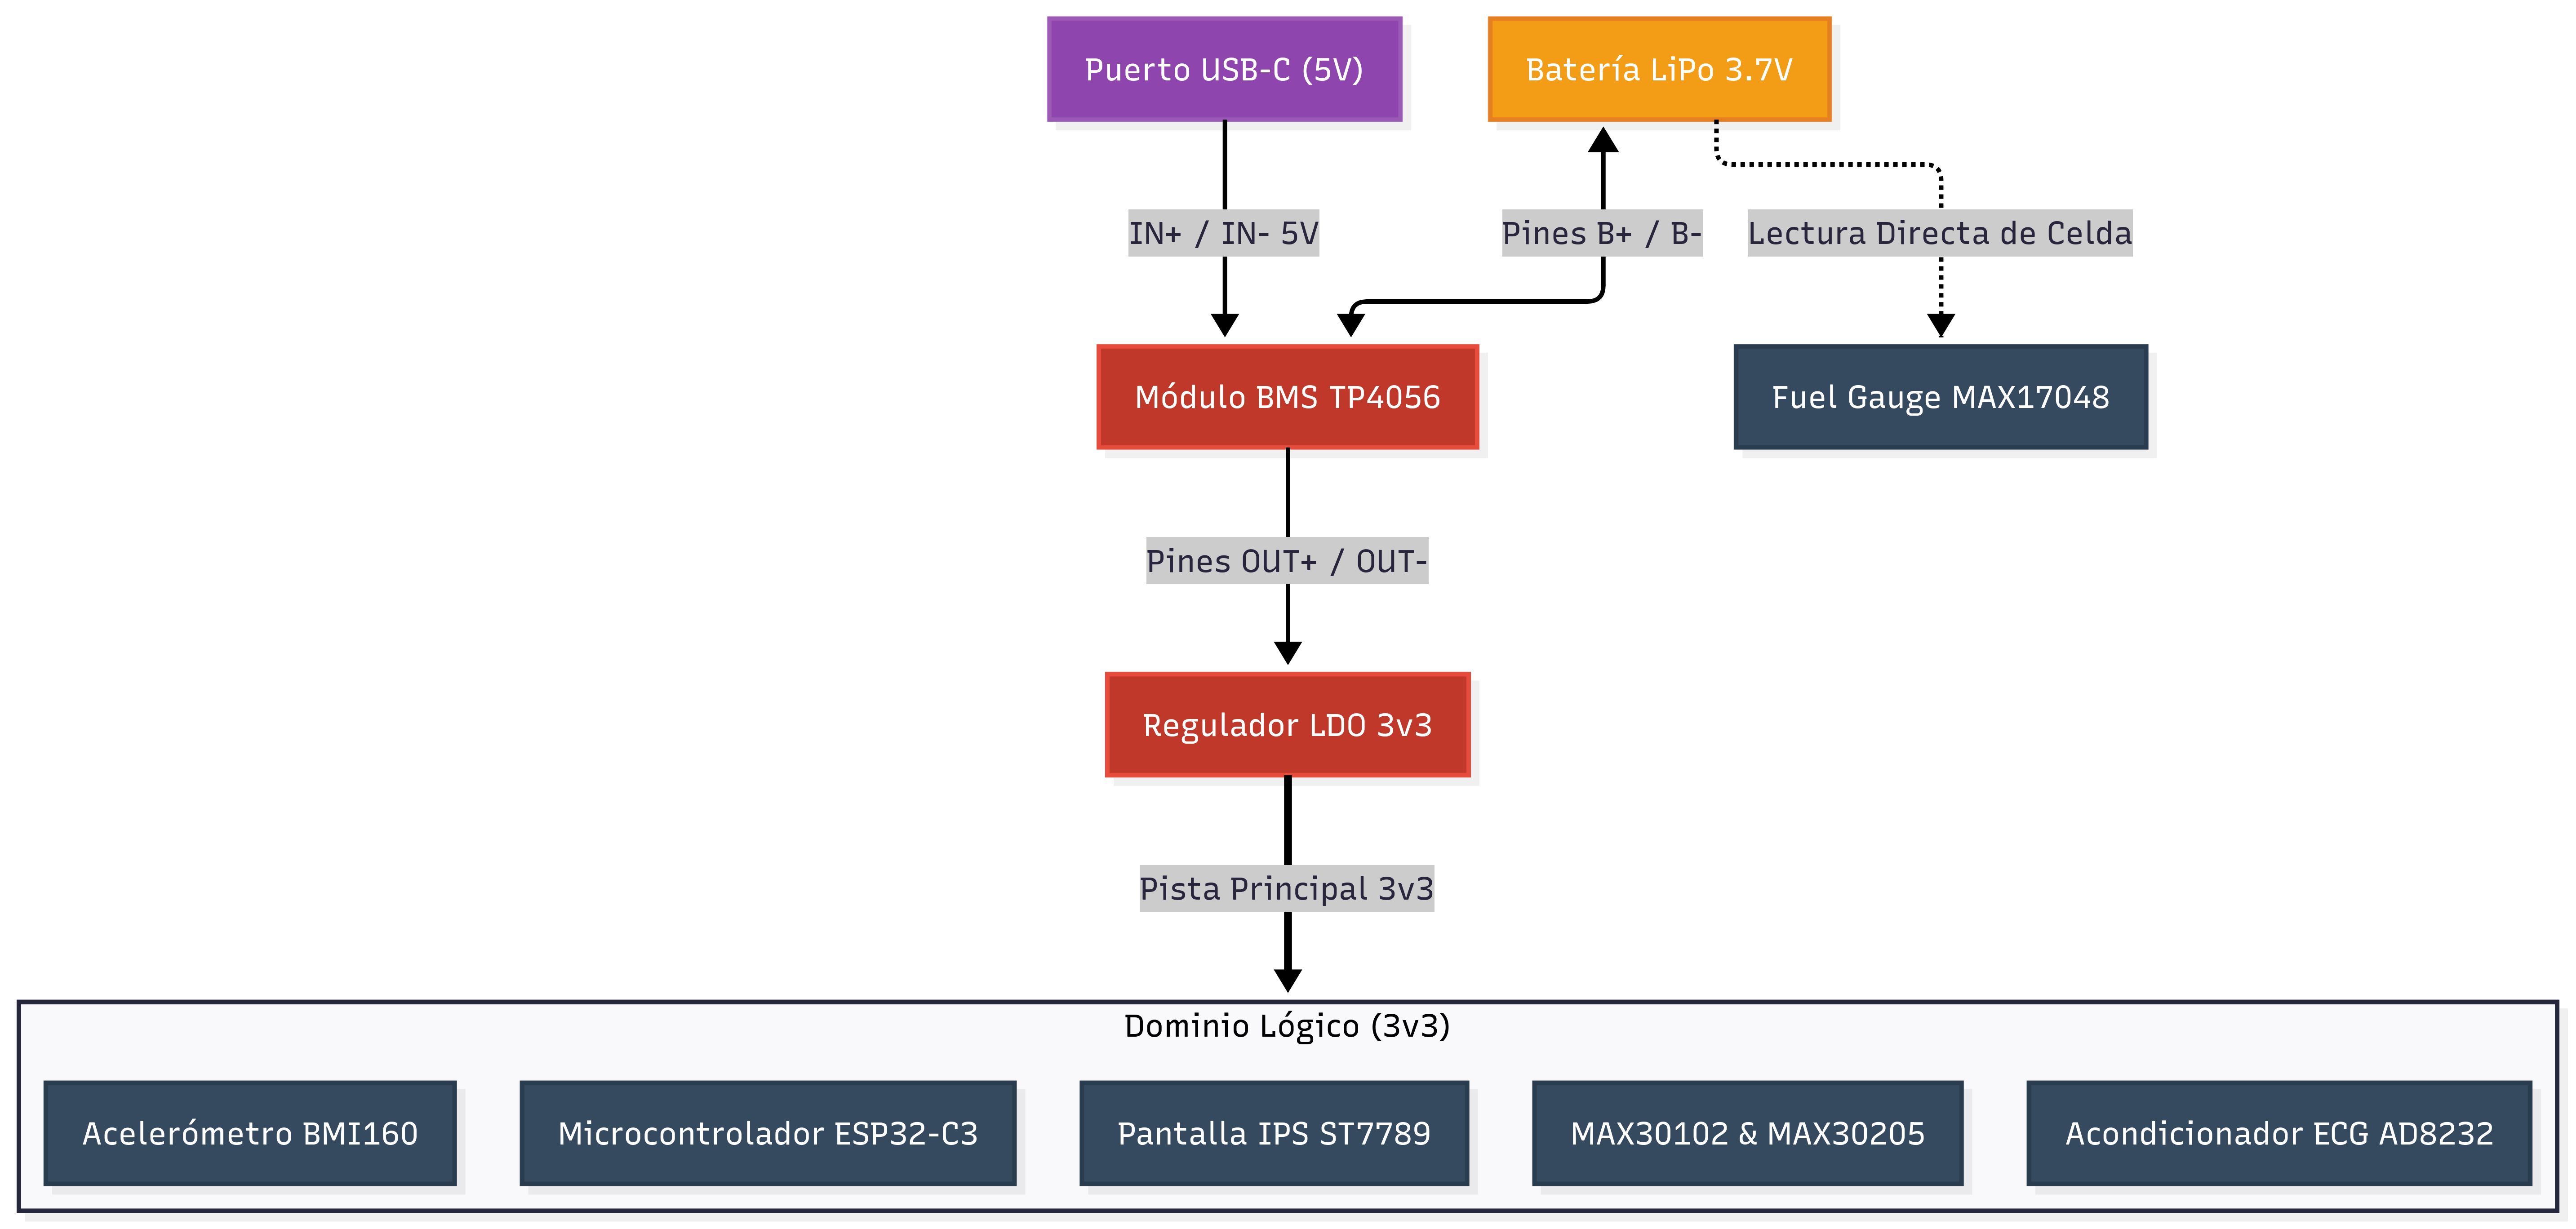
\includegraphics[width=1.0\textwidth]{img/power_diagram.png}
    \caption{Diagrama de flujo de potencia y gestión de batería del sistema SupaClock.}
    \label{fig:potencia}
\end{figure}

\begin{itemize}
    \item \textbf{Fuentes de Entrada y Gestión (BMS):} El sistema posee un funcionamiento autónomo alimentado por una batería LiPo de 3.7V. Para el proceso de recarga, se utiliza un puerto USB tipo C que suministra 5V a los pines de entrada (IN+/IN-) del módulo de gestión de batería (BMS) TP4056. Este módulo actúa como intermediario, encargándose de cargar la celda de forma segura (pines B+/B-) y aislar el circuito para protegerlo contra sobredescargas y cortocircuitos mediante el integrado DW01A.
    \item \textbf{Monitoreo Independiente (Fuel Gauge):} Para informar el nivel de carga al usuario, se ha integrado el sensor MAX17048. Este componente realiza una lectura de voltaje directa desde los terminales de la celda LiPo, operando en paralelo al BMS.
    \item \textbf{Regulación y Dominio Lógico (3.3V):} La salida de energía protegida (OUT+/OUT-) proveniente del BMS se direcciona hacia un regulador lineal (LDO). Este componente estabiliza la tensión fluctuante de la batería y establece una pista principal constante de 3.3V. Este dominio lógico unificado alimenta simultáneamente a todos los circuitos integrados del sistema: el microcontrolador central ESP32-C3 (S3 en posteriores versiones), la pantalla IPS ST7789, el acelerómetro BMI160, los biosensores MAX30102 y MAX30205, y el acondicionador de señal analógico del ECG (AD8232).
\end{itemize}
\subsection{Diagrama de señales y buses de comunicación}

La arquitectura de comunicación del \textit{SupaClock} ha sido diseñada para minimizar el uso de pines del microcontrolador, agrupar sensores de la misma naturaleza y facilitar la futura migración del ESP32-C3 al ESP32-S3 de ser necesario (más que nada por temás de potencia a la hora de probar el \textit{Machine Learning}). El flujo de datos se ilustra en la \rfigura{fig:senales}:

\begin{figure}[H]
    \centering
    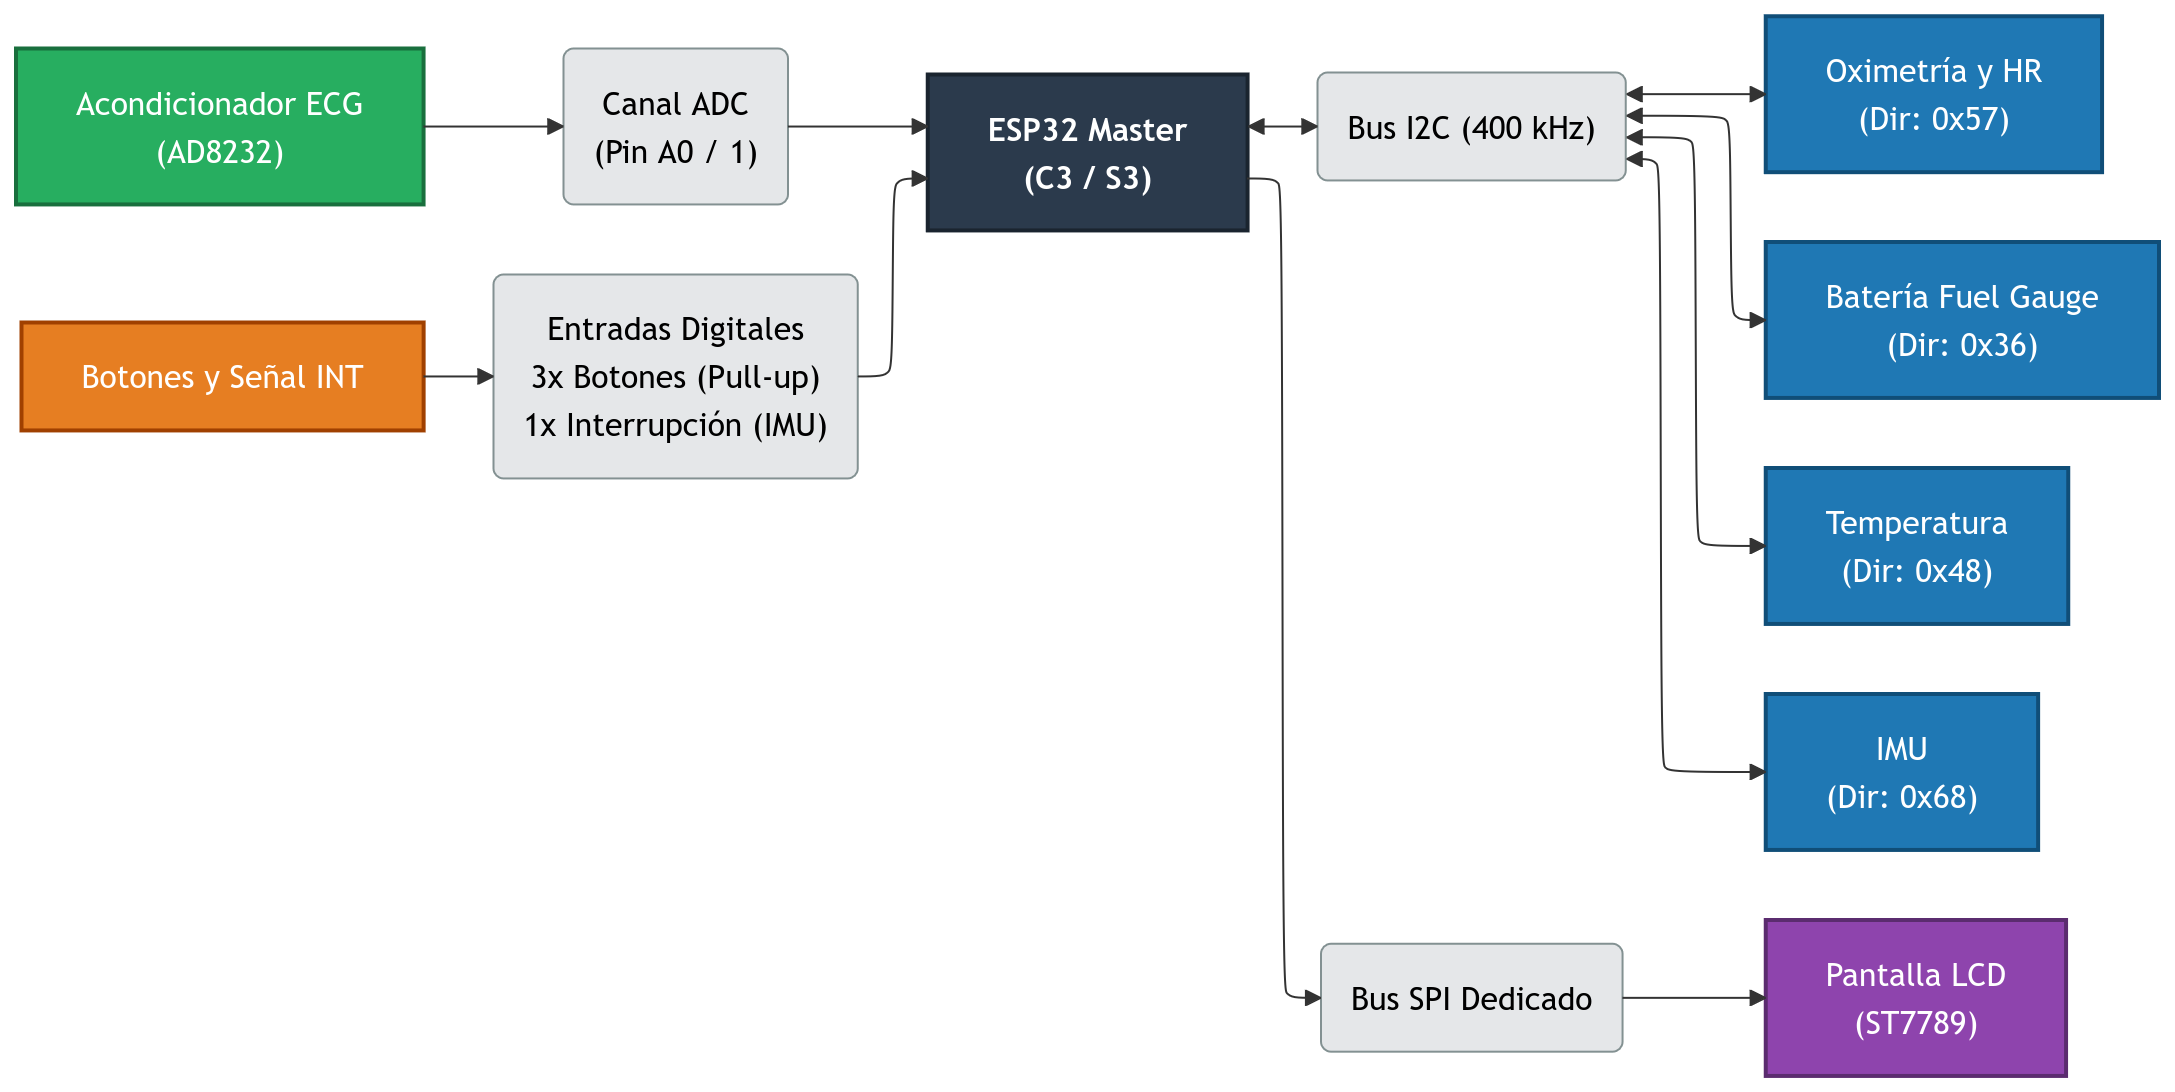
\includegraphics[width=0.9\textwidth]{img/signal_diagram.png}
    \caption{Diagrama de arquitectura de señales, buses lógicos y direcciones I2C.}
    \label{fig:senales}
\end{figure}

El sistema divide las señales en cuatro dominios principales:
\begin{itemize}
    \item \textbf{Bus I2C (Sensores):} Actúa como el bus principal de telemetría operando a 400 kHz. Agrupa el sensor de oximetría (MAX30102 - \texttt{0x57}), el monitor de batería (MAX17048 - \texttt{0x36}), el sensor de temperatura (MAX30205 - \texttt{0x48}) y la unidad inercial (BMI160 - \texttt{0x68}). El uso de este bus compartido es crítico para ahorrar puertos de I/O.
    \item \textbf{Bus SPI (Pantalla):} Un bus dedicado de alta velocidad. Está asignado al controlador ST7789 de la pantalla LCD. Solo requiere señales de salida (MOSI, Reloj, CS, DC, Reset), ya que no es necesario leer información desde la pantalla, ahorrando el pin MISO.
    \item \textbf{Canal Analógico (ECG):} La salida analógica filtrada proveniente del módulo AD8232 requiere de un conversor analógo-digital, el cual funcionará mediante la DMA. Este se conectará a un pin ADC dedicado.
    \item \textbf{Entradas Digitales (Botones e Interrupciones):} Tres líneas GPIO configuradas como entradas con resistencias \textit{pull-up} internas para los botones físicos, y un pin adicional conectado al pin \texttt{INT1} del BMI160, permitiendo despertar al microcontrolador mediante este mismo de ser necesario a futuro.
\end{itemize}

\subsubsection{Mapeo de pines y plan de migración (C3 a S3)}
El proyecto contempla el desarrollo de los primeros prototipos con la placa ESP32-C3 \textit{SuperMini} (que posee 13 GPIOs expuestos) y la migración final hacia el ESP32-S3 \textit{SuperMini} (que posee 16 GPIOs), esto es altamente probable debido a los requerimientos de \textit{Machine Learning}, pero debido al bajo costo monetario de los módulos, preferimos probar primero con el de menor consumo. Tras analizar los esquemáticos de ambas placas, se confirma que la cantidad de pines es suficiente. Aprovechando la matriz GPIO, se ha definido un mapa de pines (\rtabla{tab:pines}) que intenta mantener la compatibilidad física entre ambas arquitecturas:

\begin{table}[H]
    \centering
    \begin{tabular}{|l|c|c|l|}
        \hline
        \rowcolor[HTML]{E5E7E9}
        \textbf{Periférico / Señal} & \textbf{Pin ESP32-C3} & \textbf{Pin ESP32-S3} & \textbf{Tipo de Señal}    \\ \hline
        Bus I2C (SDA)               & GPIO 8                & GPIO 33               & Digital Bidireccional     \\ \hline
        Bus I2C (SCL)               & GPIO 9                & GPIO 34               & Digital Reloj             \\ \hline
        Pantalla SPI (MOSI)         & GPIO 6                & GPIO 6                & Digital Salida            \\ \hline
        Pantalla SPI (SCK)          & GPIO 4                & GPIO 4                & Digital Reloj             \\ \hline
        Pantalla SPI (CS)           & GPIO 5                & GPIO 5                & Digital Salida            \\ \hline
        Pantalla SPI (DC)           & GPIO 3                & GPIO 3                & Digital Salida            \\ \hline
        Pantalla SPI (RST)          & GPIO 7                & GPIO 7                & Digital Salida            \\ \hline
        ECG (AD8232 Out)            & GPIO 0 (A0)           & GPIO 1                & Analógica (ADC)           \\ \hline
        Interrupción IMU (INT1)     & GPIO 1                & GPIO 2                & Entrada Digital           \\ \hline
        Botón 1 (Seleccionar)       & GPIO 10               & GPIO 14               & Entrada Digital (Pull-up) \\ \hline
        Botón 2 (Arriba)            & GPIO 20               & GPIO 15               & Entrada Digital (Pull-up) \\ \hline
        Botón 3 (Abajo)             & GPIO 21               & GPIO 16               & Entrada Digital (Pull-up) \\ \hline
    \end{tabular}
    \caption{Mapeo definitivo de señales para placas SuperMini.}
    \label{tab:pines}
\end{table}

\subsection{Arquitectura de Firmware (FreeRTOS)}
Para gestionar la concurrencia de múltiples sensores y garantizar tiempos de ejecución deterministas, el microcontrolador ESP32 operará bajo el sistema operativo en tiempo real FreeRTOS. La arquitectura interna del dispositivo se estructurará de la siguiente manera:

\begin{itemize}
    \item \textbf{Gestión de Tareas (Multitasking):} El sistema se dividirá en tareas independientes asignadas a distintos niveles de prioridad para optimizar el uso del procesador:
          \begin{itemize}
              \item \textit{Tarea de Adquisición (Prioridad Alta):} Encargada de muestrear el ADC (para el ECG) mediante acceso directo a memoria (DMA) y leer los buses I2C a frecuencias precisas.
              \item \textit{Tarea de Procesamiento Edge (Prioridad Media):} Ejecutará el modelo de \textit{TinyML} para la clasificación de actividad y el algoritmo del contador de pasos de forma local.
              \item \textit{Tarea de Interfaz Gráfica (Prioridad Media-Baja):} Actualizará la pantalla LCD vía SPI y gestionará las interrupciones de los botones físicos para la navegación fluida.
              \item \textit{Tarea de Comunicación BLE (Prioridad Baja):} Empaquetará los datos y manejará la conexión con el teléfono móvil de forma asíncrona, evitando bloquear el sistema principal.
          \end{itemize}
    \item \textbf{Sincronización y Comunicación (IPC):} Para evitar colisiones en los buses de datos (como el bus I2C compartido por cuatro sensores biométricos), se implementarán semáforos de exclusión mutua (\textit{Mutexes}). La transferencia de datos entre la tarea de adquisición y la de procesamiento se realizará mediante colas de mensajes (\textit{Queues}), asegurando que no se pierdan muestras críticas.
    \item \textbf{Gestión Energética Activa:} El planificador de FreeRTOS se configurará en conjunto con las rutinas de bajo consumo del ESP32 (\textit{Light Sleep}). El sistema dormirá la mayor parte del tiempo y será despertado únicamente por interrupciones de hardware o temporizadores internos.
\end{itemize}

\subsubsection{Frecuencias de Muestreo y Optimización de Memoria}
Para optimizar el uso de la memoria SRAM del microcontrolador y el ancho de banda de transmisión Bluetooth, se diferenciarán las tasas de muestreo interno (\textit{hardware}) de las tasas de registro lógico:
\begin{itemize}
    \item \textbf{Sensores Dinámicos (IMU y PPG):} Muestreados internamente a frecuencias elevadas (50 a 100 Hz) para alimentar el modelo de \textit{Machine Learning} y algoritmos de biometría. Los datos crudos no serán almacenados; el microcontrolador extraerá las características en tiempo real y solo registrará en el \textit{buffer} de transmisión los resultados procesados a 1 Hz.
    \item \textbf{Sensores de Dinámica Lenta (Temperatura):} El sensor operará a 1 Hz, dada la alta inercia térmica del cuerpo humano.
    \item \textbf{Telemetría Cruda (ECG):} Durante la medición puntual, el ADC operará a 100 Hz mínimo. Estos datos sí serán almacenados de forma cruda (\textit{raw}) y transmitidos inmediatamente por BLE, delegando su procesamiento a la nube.
\end{itemize}


La \rfigura{fig:freertos_flow} presenta el diagrama de bloques del firmware, mostrando la arquitectura de tareas concurrentes bajo FreeRTOS, los periféricos de hardware conectados al microcontrolador y los mecanismos de comunicación entre procesos (IPC). Las cajas grises representan los periféricos de hardware, las cajas azules las tareas de software, las cajas amarillas las colas de mensajes (\textit{Queues}) y el círculo rojo el semáforo de exclusión mutua (\textit{Mutex}) que protege el bus I2C compartido. Las flechas continuas indican flujo de datos y las discontinuas representan interrupciones asíncronas.

\shorthandoff{>}\shorthandoff{<}
\begin{figure}[H]
    \centering
    \resizebox{\textwidth}{!}{%
        \begin{tikzpicture}[
                node distance=1.2cm and 1.5cm,
                sensor/.style={rectangle, rounded corners, draw=black, top color=white, bottom color=gray!20, text width=2.5cm, align=center, minimum height=1cm, font=\footnotesize},
                task/.style={rectangle, rounded corners, draw=black, thick, top color=white, bottom color=blue!10, text width=4cm, align=center, minimum height=1.5cm, font=\small},
                queue/.style={rectangle, draw=black, fill=yellow!20, text width=2.5cm, align=center, minimum height=0.8cm, font=\footnotesize\ttfamily},
                mutex/.style={circle, draw=black, fill=red!20, inner sep=2pt, font=\footnotesize\bfseries},
                arrow/.style={thick, ->, >=stealth},
                dashed_arrow/.style={thick, dashed, ->, >=stealth},
                legend/.style={rectangle, draw=black!50, fill=white, inner sep=5pt, font=\scriptsize}
            ]%
            % Nodos de Hardware
            \node[sensor] (adc) {ADC / DMA\\(ECG 100Hz)};
            \node[sensor, below=of adc] (i2c) {Bus I2C\\(IMU, PPG, Temp)};
            \node[sensor, below=of i2c] (btns) {Botones físicos\\(Interrupciones)};
            %
            % Mutex
            \node[mutex, right=0.5cm of i2c] (mut) {M};
            %
            % Nodos de Tareas FreeRTOS
            \node[task, right=1.5cm of adc] (t_acq) {\textbf{Tarea Adquisición}\\ \textit{Prioridad: Alta}\\(Muestreo de sensores)};
            \node[task, below=1cm of t_acq] (t_proc) {\textbf{Tarea Procesamiento}\\ \textit{Prioridad: Media}\\(TinyML, Pasos)};
            \node[task, below=1cm of t_proc] (t_gui) {\textbf{Tarea Interfaz Gráfica}\\ \textit{Prioridad: Media-Baja}\\(Actualización SPI)};
            \node[task, right=1.5cm of t_proc] (t_ble) {\textbf{Tarea Com. BLE}\\ \textit{Prioridad: Baja}\\(Empaquetado y envío)};
            %
            % Colas (Queues)
            \node[queue, right=0.3cm of t_acq, yshift=-1cm] (q_data) {Queue: Datos};
            \node[queue, right=0.3cm of t_proc, yshift=-1cm] (q_ble) {Queue: Tx BLE};
            %
            % Background / Boundary para ESP32
            \begin{scope}[on background layer]
                \node[rectangle, draw=black!50, dashed, inner sep=0.5cm, fit=(adc) (i2c) (btns) (t_acq) (t_proc) (t_gui) (t_ble) (q_data) (q_ble) (mut), fill=black!2] (esp32) {};
                \node[anchor=north west, font=\bfseries] at (esp32.north west) {Microcontrolador ESP32 (FreeRTOS)};
            \end{scope}
            %
            % Conexiones Hardware -> Tareas
            \draw[arrow] (adc) -- (t_acq);
            \draw[arrow] (i2c) -- (mut) -- (t_acq);
            \draw[dashed_arrow] (btns) -- node[above, font=\scriptsize] {ISR} (t_gui);
            %
            % Conexiones entre Tareas (IPC)
            \draw[arrow] (t_acq) |- (q_data);
            \draw[arrow] (q_data) -| (t_proc);
            \draw[arrow] (t_proc) |- (q_ble);
            \draw[arrow] (q_ble) -| (t_ble);
            %
            % Conexiones de visualización
            \draw[arrow] (t_proc) -- (t_gui);
            %
            % Salidas externas
            \node[sensor, right=1.5cm of t_ble] (phone) {Smartphone\\(App Gateway)};
            \node[sensor, right=1.5cm of t_gui] (lcd) {Pantalla LCD\\(ST7789)};
            %
            \draw[arrow, blue, thick] (t_ble) -- node[above, font=\scriptsize] {BLE} (phone);
            \draw[arrow] (t_gui) -- node[above, font=\scriptsize] {SPI} (lcd);
            %
            % === LEYENDA ===
            \node[legend, below=0.5cm of esp32] (leg) {
                \begin{tabular}{cl}
                    \tikz\draw[fill=gray!20] (0,0) rectangle (0.3,0.2);   & Periférico de hardware       \\
                    \tikz\draw[fill=blue!10] (0,0) rectangle (0.3,0.2);   & Tarea FreeRTOS               \\
                    \tikz\draw[fill=yellow!20] (0,0) rectangle (0.3,0.2); & Cola de mensajes (Queue)     \\
                    \tikz\draw[fill=red!20] (0,0) circle (0.1);           & Mutex (exclusión mutua)      \\
                    \tikz\draw[thick, ->] (0,0.1) -- (0.4,0.1);           & Flujo de datos               \\
                    \tikz\draw[thick, dashed, ->] (0,0.1) -- (0.4,0.1);   & Interrupción asíncrona (ISR) \\
                    \tikz\draw[blue, thick, ->] (0,0.1) -- (0.4,0.1);     & Enlace BLE inalámbrico       \\
                \end{tabular}
            };
        \end{tikzpicture}%
    }
    \caption{Diagrama de bloques del firmware y gestión de tareas en FreeRTOS.}
    \label{fig:freertos_flow}
\end{figure}
\shorthandon{>}\shorthandon{<}

\subsection{Arquitectura de Ecosistema (App y Servidor)}
El dispositivo actuará como un nodo de adquisición en el borde (\textit{Edge}), delegando el almacenamiento histórico y el análisis profundo a una arquitectura externa compuesta por una Aplicación Móvil y un backend en la nube.

\begin{itemize}
    \item \textbf{Estrategia de Transmisión (BLE):} Para optimizar el consumo energético, la transmisión Bluetooth Low Energy (BLE) operará en dos modalidades. La telemetría continua (pasos, temperatura, SpO2, actividad) se enviará a la aplicación móvil en paquetes consolidados de forma periódica. Para la medición del electrocardiograma, se abrirá un canal de alto rendimiento que transmitirá los datos a 100 Hz en tiempo real durante los 30 segundos de captura.
    \item \textbf{Aplicación Móvil (Android):} Funcionará como el enlace principal o \textit{Gateway}. Se encargará de emparejarse con el dispositivo, visualizar el resumen en tiempo real, calibrar métricas del usuario y subir los paquetes de datos al servidor.
    \item \textbf{Backend Principal (Firebase):} Durante las primeras fases de desarrollo, se utilizará el ecosistema de Firebase. \textit{Cloud Firestore} almacenará los perfiles y métricas históricas, mientras que el procesamiento pesado se ejecutará mediante \textit{Cloud Functions} utilizando Python. Esto asegura alta disponibilidad y un despliegue rápido.
    \item \textbf{Proyección a Servidor Propio (Edge Server):} Como objetivo extendido, y sujeto a la holgura en la Carta Gantt, se contempla la migración del backend a un servidor propio gestionado mediante una Raspberry Pi 3B+. Esta arquitectura \textit{On-Premise} (utilizando una API propia, bases de datos de series de tiempo e interfaces como Grafana) eliminaría la dependencia de servicios externos y maximizaría la privacidad de los datos biométricos.
\end{itemize}

La \rfigura{fig:ecosystem_flow} ilustra esta arquitectura de ecosistema. En el diagrama, las flechas azules representan la telemetría continua enviada a baja frecuencia (1 Hz), mientras que las flechas rojas indican el canal de alta velocidad para la transmisión de datos crudos de ECG (100 Hz). Las cajas verdes corresponden a dispositivos físicos, las azules a la aplicación de software y las naranjas al ecosistema en la nube. El nodo punteado en púrpura representa la proyección futura del servidor local.

\shorthandoff{>}\shorthandoff{<}
\begin{figure}[H]
    \centering
    \resizebox{\textwidth}{!}{%
        \begin{tikzpicture}[
                node distance=1.5cm and 2cm,
                device/.style={rectangle, rounded corners, draw=black, thick, top color=white, bottom color=green!10, text width=3cm, align=center, minimum height=1.5cm, font=\small\bfseries},
                app/.style={rectangle, rounded corners, draw=black, thick, top color=white, bottom color=blue!10, text width=3cm, align=center, minimum height=1.5cm, font=\small\bfseries},
                cloud/.style={ellipse, draw=black, thick, top color=white, bottom color=orange!10, text width=3.5cm, align=center, minimum height=2cm, font=\small},
                db/.style={cylinder, shape border rotate=90, aspect=0.25, draw=black, thick, top color=white, bottom color=orange!20, text width=2.5cm, align=center, minimum height=2cm, font=\footnotesize},
                func/.style={rectangle, draw=black, dashed, fill=gray!10, text width=3.5cm, align=center, minimum height=1.5cm, font=\footnotesize},
                arrow/.style={thick, ->, >=stealth},
                double_arrow/.style={thick, <->, >=stealth},
                legend/.style={rectangle, draw=black!50, fill=white, inner sep=5pt, font=\scriptsize}
            ]%
            % Nodos Principales
            \node[device] (watch) {SupaClock\\(Nodo Edge)};
            \node[app, right=3.5cm of watch] (android) {Aplicación Móvil\\(Gateway Android)};
            %
            % Nodos de Nube
            \node[cloud, right=2.5cm of android] (firebase) {\textbf{Ecosistema Firebase}};
            \node[db, right=1cm of firebase, yshift=1.5cm] (firestore) {Cloud Firestore\\(Perfiles)};
            \node[func, right=1cm of firebase, yshift=-1.5cm] (functions) {\textbf{Cloud Functions}\\(Python)\\ \textit{Algoritmo ECG}};
            %
            % Nodo Raspberry (Futuro)
            \node[device, bottom color=purple!10, dashed, below=2cm of android] (rpi) {Raspberry Pi 3B+\\(Edge Server)};
            %
            % Conexiones BLE
            \draw[arrow, blue] ([yshift=0.5cm]watch.east) -- node[above, font=\scriptsize, text=black, align=center] {BLE (1 Hz)\\Telemetría Continua} ([yshift=0.5cm]android.west);
            \draw[arrow, red] ([yshift=-0.5cm]watch.east) -- node[below, font=\scriptsize, text=black, align=center] {BLE (100 Hz)\\ECG Crudo} ([yshift=-0.5cm]android.west);
            %
            % Conexiones App -> Nube
            \draw[double_arrow] (android) -- node[above, font=\scriptsize] {Wi-Fi / 4G} (firebase);
            %
            % Conexiones internas nube
            \draw[arrow] (firebase) -- (firestore);
            \draw[arrow] (firebase) -- (functions);
            \draw[arrow, dashed] (functions) -- node[right, font=\scriptsize] {Actualiza BPM} (firestore);
            %
            % Conexión Futura
            \draw[double_arrow, dashed, purple] (android) -- node[right, font=\scriptsize] {Proyección local} (rpi);
            %
            % === LEYENDA ===
            \node[legend, below=1cm of watch, xshift=3cm] (leg) {
                \begin{tabular}{cl}
                    \tikz\draw[fill=green!10] (0,0) rectangle (0.3,0.2);          & Dispositivo físico      \\
                    \tikz\draw[fill=blue!10] (0,0) rectangle (0.3,0.2);           & Aplicación de software  \\
                    \tikz\draw[fill=orange!10] (0,0) rectangle (0.3,0.2);         & Servicio en la nube     \\
                    \tikz\draw[fill=purple!10, dashed] (0,0) rectangle (0.3,0.2); & Proyección futura       \\
                    \tikz\draw[blue, thick, ->] (0,0.1) -- (0.4,0.1);             & BLE: Telemetría (1 Hz)  \\
                    \tikz\draw[red, thick, ->] (0,0.1) -- (0.4,0.1);              & BLE: ECG crudo (100 Hz) \\
                    \tikz\draw[purple, thick, dashed, <->] (0,0.1) -- (0.4,0.1);  & Enlace futuro           \\
                \end{tabular}
            };
        \end{tikzpicture}%
    }
    \caption{Arquitectura de ecosistema: flujo de datos desde el dispositivo \textit{Edge} hacia la aplicación móvil y el backend en la nube.}
    \label{fig:ecosystem_flow}
\end{figure}
\shorthandon{>}\shorthandon{<}

\subsubsection{Algoritmos de Procesamiento de Señales (ECG en Servidor)}
Para la estimación de la frecuencia cardíaca a partir de la señal del AD8232, se implementará el algoritmo de \textbf{Pan-Tompkins} de manera asíncrona en el servidor (ej. funciones nativas en Python):
\begin{enumerate}
    \item \textbf{Filtrado Digital Pasabanda:} Atenuación del ruido de alta frecuencia (interferencia electromagnética) y eliminación de la deriva de la línea base (\textit{baseline wander}).
    \item \textbf{Procesamiento Morfológico:} Aplicación de un filtro derivativo y función de cuadratura para resaltar la pendiente aguda del complejo QRS.
    \item \textbf{Detección de Picos R:} Integración de ventana móvil combinada con umbrales adaptativos (\textit{adaptive thresholding}) para identificar el instante exacto de cada latido.
    \item \textbf{Cálculo de Métricas:} Evaluación de la distancia temporal entre picos consecutivos (intervalos R-R) para calcular los latidos por minuto (BPM) y evaluar la Variabilidad de la Frecuencia Cardíaca (HRV).
\end{enumerate}


\section{Bosquejo de la solución}

La \rfigura{fig:bosquejo} presenta el bosquejo preliminar del prototipo SupaClock, el cual ilustra las principales vistas y dimensiones del dispositivo. Desde la vista cenital se aprecia la interfaz del usuario con la pantalla principal y los íconos de navegación. En la vista frontal se observan los tres botones físicos ubicados en el costado derecho, los cuales cumplirán las funciones de navegación (arriba/abajo) y selección/acción. La vista lateral derecha muestra la ubicación de los electrodos de contacto seco para la medición de ECG, posicionados en la zona más cercana a la mano del usuario. Finalmente, la vista posterior exhibe el puerto USB-C de carga y la correa ajustable. Las cotas indicadas corresponden a las dimensiones máximas de diseño: largo $\leq$ 80 mm, ancho $\leq$ 50 mm y altura $\leq$ 30 mm.

\begin{figure}[H]
    \centering
    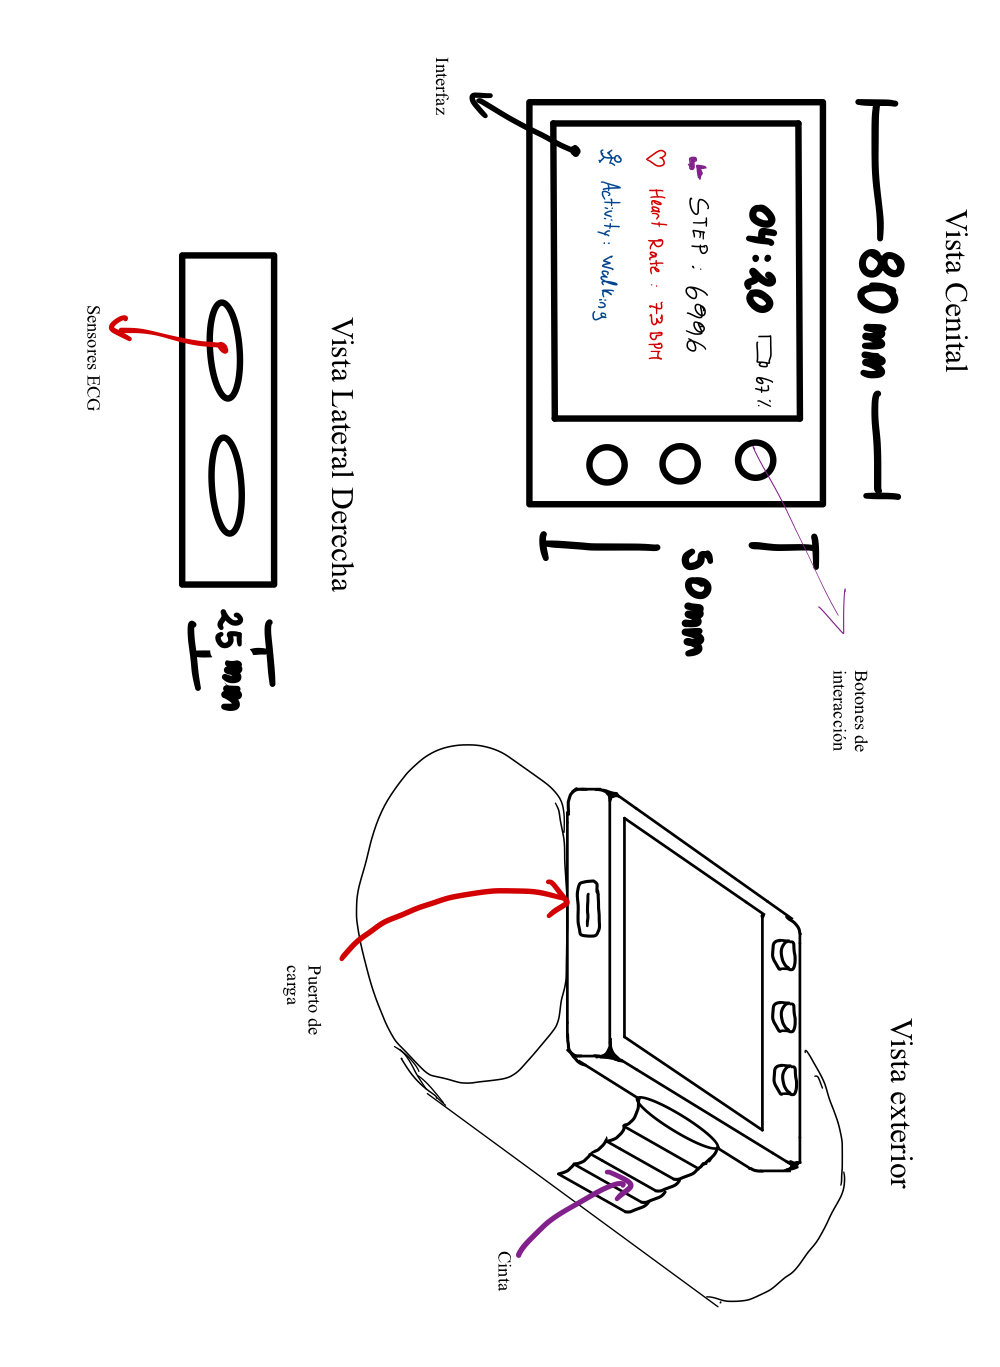
\includegraphics[width=0.5\textwidth, angle = 90]{img/Bosquejo.png}
    \caption{Bosquejo preliminar del prototipo SupaClock con vistas cenital, frontal, lateral y posterior.}
    \label{fig:bosquejo}
\end{figure}
% ==========================================
% 3. PLANIFICACIÓN
% ==========================================
% ==========================================
% 4. IMPLEMENTACIÓN Y RESULTADOS
% ==========================================
\section{Metodología de trabajo}
Para el proyecto se colocarán los avances que cada persona va realizando en una tarea en particular, para esto se utilizará la plataforma Notion y Git (github), en las cuales se organiza la creación y ejecución de tareas, registran los avances de los proyectos de código respectivamente. También realizaremos trabajo presencial en conjunto al menos cuatro módulos a la semana se realizarán jornadas remotas orientadas principalmente para los bloques de programación y escritura de código.
\subsection{Áreas y roles}

El desarrollo del proyecto se divide en tres áreas principales: Hardware, Software y Procesamiento, e Interfaz y Sistema. Esta división permite un trabajo modular, paralelo y eficiente, facilitando la integración final del sistema.

\subsubsection{Área 1: Hardware}

La primera área es \textbf{Hardware}, esta contempla los sensores, el diseño de la PCB, el manejo físico de la energía y la integración de estos bloques. Dentro de sus tareas se encuentran la selección de componentes, diseño esquemático, diseño de PCB, integración física, diseño del sistema de alimentación y pruebas eléctricas.

A cargo de esta área se encuentra \textbf{Benjamín Sepúlveda}, encargado de registrar los avances asociados a esta rama.

Los roles asociados a esta área son:
\begin{itemize}
    \item \textbf{Diseñador de Hardware}: encargado del diseño completo del sistema, tanto a nivel físico como eléctrico.
    \item \textbf{Energía}: responsable del manejo de la batería, sistema de carga y optimización del consumo energético.
    \item \textbf{Electrónica}: encargado de la conexión entre sensores y microcontrolador, además del debug de hardware.
\end{itemize}

\subsubsection{Área 2: Software y Procesamiento}

La segunda área es \textbf{Software y Procesamiento}, la cual cubre firmware, algoritmos y machine learning. Dentro de sus tareas se encuentra la lectura de sensores y su comunicación, filtrado de señales de ECG, implementación del contador de pasos y gestión del sistema operativo FreeRTOS.

A cargo de esta área se encuentra \textbf{Pablo Uribe}, encargado de la gestión de los procesos asociados.

Los roles asociados a esta área son:
\begin{itemize}
    \item \textbf{Firmware}: encargado de la arquitectura del código, implementación de drivers y comunicación con los sensores.
    \item \textbf{Procesamiento y Señales}: responsable del filtrado de señales (ECG), cálculo de métricas fisiológicas y desarrollo del contador de pasos.
    \item \textbf{Machine Learning}: encargado de implementar y optimizar el modelo de clasificación de actividades en el dispositivo (TinyML), considerando restricciones de consumo y latencia.
\end{itemize}

\subsubsection{Área 3: Interfaz y Sistema}

La tercera área es \textbf{Interfaz y Sistema}, la cual contempla la interacción con el usuario, visualización de datos y comunicación externa del dispositivo. Dentro de sus tareas se encuentra el diseño de la interfaz gráfica (GUI), navegación del sistema, despliegue de métricas en pantalla, implementación de comunicación inalámbrica (BLE/WiFi) y la integración completa del sistema.

A cargo de esta área se encuentra \textbf{Tomás Avendaño}, responsable de coordinar la integración final del dispositivo.

Los roles asociados a esta área son:
\begin{itemize}
    \item \textbf{Desarrollador UI/UX}: encargado del diseño e implementación de la interfaz gráfica, asegurando una experiencia de usuario clara e intuitiva.
    \item \textbf{Comunicaciones}: responsable de la transmisión de datos mediante BLE/WiFi hacia dispositivos externos o plataformas externas.
    \item \textbf{Integrador de Sistema}: encargado de la integración de hardware, software e interfaz, además de realizar pruebas completas del sistema.
\end{itemize}


\subsection{Trabajo colaborativo}

El desarrollo del proyecto se basa en una metodología de trabajo colaborativo, donde cada área cuenta con un encargado responsable de su correcta ejecución. Sin embargo, esto no implica que el trabajo recaiga exclusivamente en dicha persona, sino que su rol principal es coordinar, organizar y supervisar las tareas dentro de su área.

Cada encargado deberá distribuir los roles definidos previamente entre los integrantes del equipo, asignando responsabilidades específicas de acuerdo a las necesidades del proyecto y a las habilidades de cada miembro. De esta forma, se busca asegurar una carga de trabajo equilibrada, fomentar la especialización en distintas áreas y mejorar la eficiencia del desarrollo.

Adicionalmente, se promoverá la colaboración entre áreas, especialmente en etapas de integración, donde será necesario coordinar esfuerzos entre hardware, software e interfaz para asegurar el correcto funcionamiento del sistema completo. Este enfoque permite reducir errores de integración y facilita la detección temprana de problemas.

\subsection{Asignación de tareas}

La asignación de tareas se realizará de manera dinámica y progresiva, en función del avance del proyecto y los hitos establecidos en la planificación. Cada área definirá sus propias tareas específicas, las cuales serán desglosadas en actividades más pequeñas y manejables.

Para la gestión de estas tareas se utilizarán herramientas colaborativas como Notion y GitHub, las cuales permitirán llevar un seguimiento continuo del progreso, asignar responsables, establecer plazos y documentar los avances realizados. Cada tarea contará con un responsable principal, quien será el encargado de su ejecución, sin perjuicio de recibir apoyo de otros integrantes cuando sea necesario.

Asimismo, se establecerán instancias periódicas de revisión, donde cada área reportará sus avances, dificultades y próximos pasos. Esto permitirá mantener una visión global del estado del proyecto, facilitar la toma de decisiones y asegurar el cumplimiento de los objetivos planteados.

Finalmente, la asignación de tareas será flexible, permitiendo reasignaciones en caso de sobrecarga de trabajo, dificultades técnicas o cambios en los requerimientos del proyecto, garantizando así la continuidad y adaptabilidad del desarrollo.

\section{Objetivos a cumplir}

El desarrollo del proyecto SupaClock tiene como objetivo principal el diseño e implementación de un dispositivo wearable funcional, capaz de adquirir, procesar y visualizar variables biométricas en tiempo real, cumpliendo con los requerimientos de portabilidad, autonomía energética y robustez del sistema.

Para alcanzar este objetivo general, se plantean los siguientes objetivos específicos:

\begin{itemize}
    \item Diseñar e implementar el sistema de adquisición de señales biométricas, incluyendo sensores de frecuencia cardíaca, SpO2, temperatura, aceleración y ECG.
    \item Desarrollar la arquitectura de procesamiento basada en un microcontrolador ESP32, capaz de ejecutar algoritmos de filtrado, análisis de señales y clasificación de actividad mediante Machine Learning.
    \item Implementar una interfaz gráfica que permita visualizar en tiempo real las métricas obtenidas, junto con un sistema de navegación intuitivo.
    \item Diseñar un sistema de alimentación autónomo basado en batería LiPo, incluyendo gestión de carga, regulación de voltaje y monitoreo de batería.
    \item Integrar todos los subsistemas en una PCB funcional, asegurando la correcta comunicación entre módulos y la estabilidad del sistema.
    \item Validar experimentalmente el funcionamiento del dispositivo mediante pruebas de sensores, consumo energético y desempeño del sistema completo.
\end{itemize}

\subsection{Hitos}

El desarrollo del proyecto se organiza en distintos hitos de avance, los cuales permiten evaluar el progreso del sistema de manera incremental.

\subsubsection{Hito 5\%: Definición y planificación inicial}

En esta etapa se establece la base conceptual del proyecto. Se espera contar con:
\begin{itemize}
    \item Prueba preliminar de componentes por separado.
    \item Crear la base de datos en Firebase.
    \item Crear el servidor en Firebase.
    \item Crear el repositorio en GitHub.
\end{itemize}

\subsubsection{Hito 25\%: Validación de subsistemas iniciales}

En este punto se busca validar el funcionamiento básico de los principales módulos del sistema:
\begin{itemize}
    \item Implementación del bloque de energía (BMS y regulación).
    \item Integración inicial de sensores.
    \item Pruebas preliminares de adquisición de datos.
    \item Primera integración con microcontrolador de los sensores en conjunto.
    \item Validación básica de algoritmos.
\end{itemize}

\subsubsection{Hito 60\%: Integración funcional del sistema}

En esta etapa el sistema comienza a operar de manera integrada:
\begin{itemize}
    \item Diseño e implementación de la PCB.
    \item Integración de sensores en la PCB.
    \item Desarrollo de la interfaz gráfica en pantalla.
    \item Implementación de algoritmos de procesamiento (ECG, pasos).
    \item Integración de comunicación inalámbrica (Bluetooth).
    \item Pruebas funcionales del sistema completo.
\end{itemize}

\subsubsection{Hito 90\%: Validación avanzada y optimización}

En esta fase el sistema se encuentra prácticamente completo y se enfoca en su validación:
\begin{itemize}
    \item Pruebas biométricas completas en condiciones reales.
    \item Optimización del consumo energético.
    \item Ajuste de algoritmos de Machine Learning.
    \item Validación de estabilidad del sistema.
    \item Integración final de hardware, software e interfaz.
\end{itemize}

\subsubsection{Hito 100\%: Entrega final}

Corresponde a la finalización del proyecto:
\begin{itemize}
    \item Dispositivo completamente funcional e integrado.
    \item Validación final del sistema.
    \item Documentación completa del proyecto.
    \item Presentación final del prototipo.
\end{itemize}

La \rfigura{fig:gantt} presenta la carta Gantt del proyecto, la cual desglosa las actividades planificadas para cada hito en un horizonte temporal que abarca el semestre académico completo. Las barras de color representan la duración estimada de cada tarea, permitiendo visualizar el paralelismo entre actividades de hardware, software e interfaz, así como identificar las dependencias críticas entre subsistemas.

\begin{figure}[H]
    \centering
    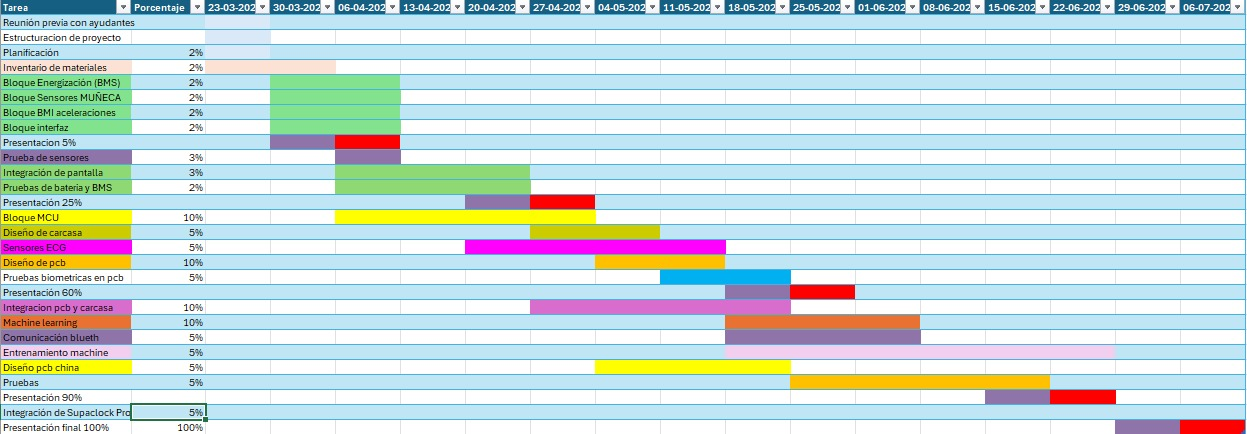
\includegraphics[width=1\textwidth]{img/Carta Gantt.jpeg}
    \caption{Carta Gantt del proyecto SupaClock con la planificación temporal de actividades por hito.}
    \label{fig:gantt}
\end{figure}





% ==========================================
% 5. PRESUPUESTO
% ==========================================
\section{Presupuesto estimado}

La \rtabla{tab:bom} presenta el listado de materiales (\textit{Bill of Materials}, BOM) con el costo de los componentes principales del prototipo. Los precios corresponden a las transacciones reales realizadas a través de la plataforma AliExpress durante marzo de 2026, los cuales \textbf{ya incluyen el 19\% correspondiente al IVA de importación}, junto a estimaciones conservadoras para los demás componentes genéricos. Cabe destacar que la fabricación de la placa de desarrollo prototipo es otorgada gratuitamente por el laboratorio; no obstante, para el objetivo extendido (\textit{Bonus} "Versión Pro"), se contempla la manufactura externa (JLCPCB o PCBWay) estimando un valor de \$30.000 CLP con envío incluido.

\begin{table}[H]
    \centering
    \renewcommand{\arraystretch}{1.3}
    \begin{tabular}{|l|c|c|r|}
        \hline
        \rowcolor[HTML]{E5E7E9}
        \textbf{Componente}           & \textbf{Cantidad} & \textbf{Referencia}  & \textbf{Costo (CLP)} \\ \hline
        ESP32-C3 SuperMini            & 3                 & MCU principal        & \$8.211              \\ \hline
        ESP32-S3 SuperMini            & 1                 & MCU migración        & \$3.500              \\ \hline
        Módulo de expansión ESP32-C3  & 1                 & Soporte desarrollo   & \$2.235              \\ \hline
        MAX30102 (Módulo PPG)         & 2                 & SpO2 / HR            & \$3.853              \\ \hline
        MAX30205 (Sensor Temp.)       & 1                 & Temperatura clínica  & \$5.949              \\ \hline
        AD8232 (Módulo ECG)           & 1                 & Electrocardiograma   & \$3.500              \\ \hline
        BMI160 (Módulo IMU)           & 2                 & Acelerómetro + Giro  & \$3.204              \\ \hline
        MAX17048 (Fuel Gauge)         & 1                 & Monitor de batería   & \$3.000              \\ \hline
        Módulo Cargador TP4056 Type-C & 1                 & Carga y protección   & \$1.142              \\ \hline
        ME6211 / AP2112K (LDO 3.3V)   & 1                 & Regulador de voltaje & \$300                \\ \hline
        Pantalla IPS LCD 1.69" ST7789 & 1                 & Display principal    & \$3.195              \\ \hline
        Pantalla TFT LCD 1.3"         & 1                 & Display alternativo  & \$2.059              \\ \hline
        Conectores 24PIN FPC          & 10                & Interfaz pantallas   & \$2.161              \\ \hline
        Batería LiPo 3.7V 400 mAh     & 1                 & Alimentación         & \$3.000              \\ \hline
        Pulsadores táctiles SMD       & 50                & Botones navegación   & \$2.248              \\ \hline
        Conector USB-C hembra         & 1                 & Puerto de carga      & \$500                \\ \hline
        Pernos M3                     & 10                & Contactos ECG        & \$2.264              \\ \hline
        Componentes pasivos (R, C)    & ---               & Varios               & \$1.000              \\ \hline
        Filamento PLA (carcasa 3D)    & ---               & Impresión 3D         & \$2.000              \\ \hline
        PCB prototipo                 & 1                 & FabLab               & Gratis               \\ \hline
        \rowcolor[HTML]{D5F5E3}
        \textbf{Subtotal (Prototipo)} & ---               & ---                  & \textbf{\$53.321}    \\ \hline
        PCB SMD (JLCPCB/PCBWay)       & 1                 & Versión Pro (Bonus)  & \$30.000             \\ \hline
        \rowcolor[HTML]{ABEBC6}
        \textbf{Total con Bonus}      & ---               & ---                  & \textbf{\$83.321}    \\ \hline
    \end{tabular}
    \caption{Bill of Materials (BOM) con precios reales de adquisición (IVA incl.) para componentes críticos.}
    \label{tab:bom}
\end{table}


% ==========================================
% 6. REFERENCIAS
% ==========================================
\section{Referencias}

\bibliographystyle{unsrtnat}
\bibliography{ref}


\end{document}